\documentclass[../main.tex]{subfiles}

\graphicspath{../images/}

\begin{document}

\section{Vector Analysis}
\barh 

\paragraph{1.1}
\begin{figure}[ht]
    \centering
    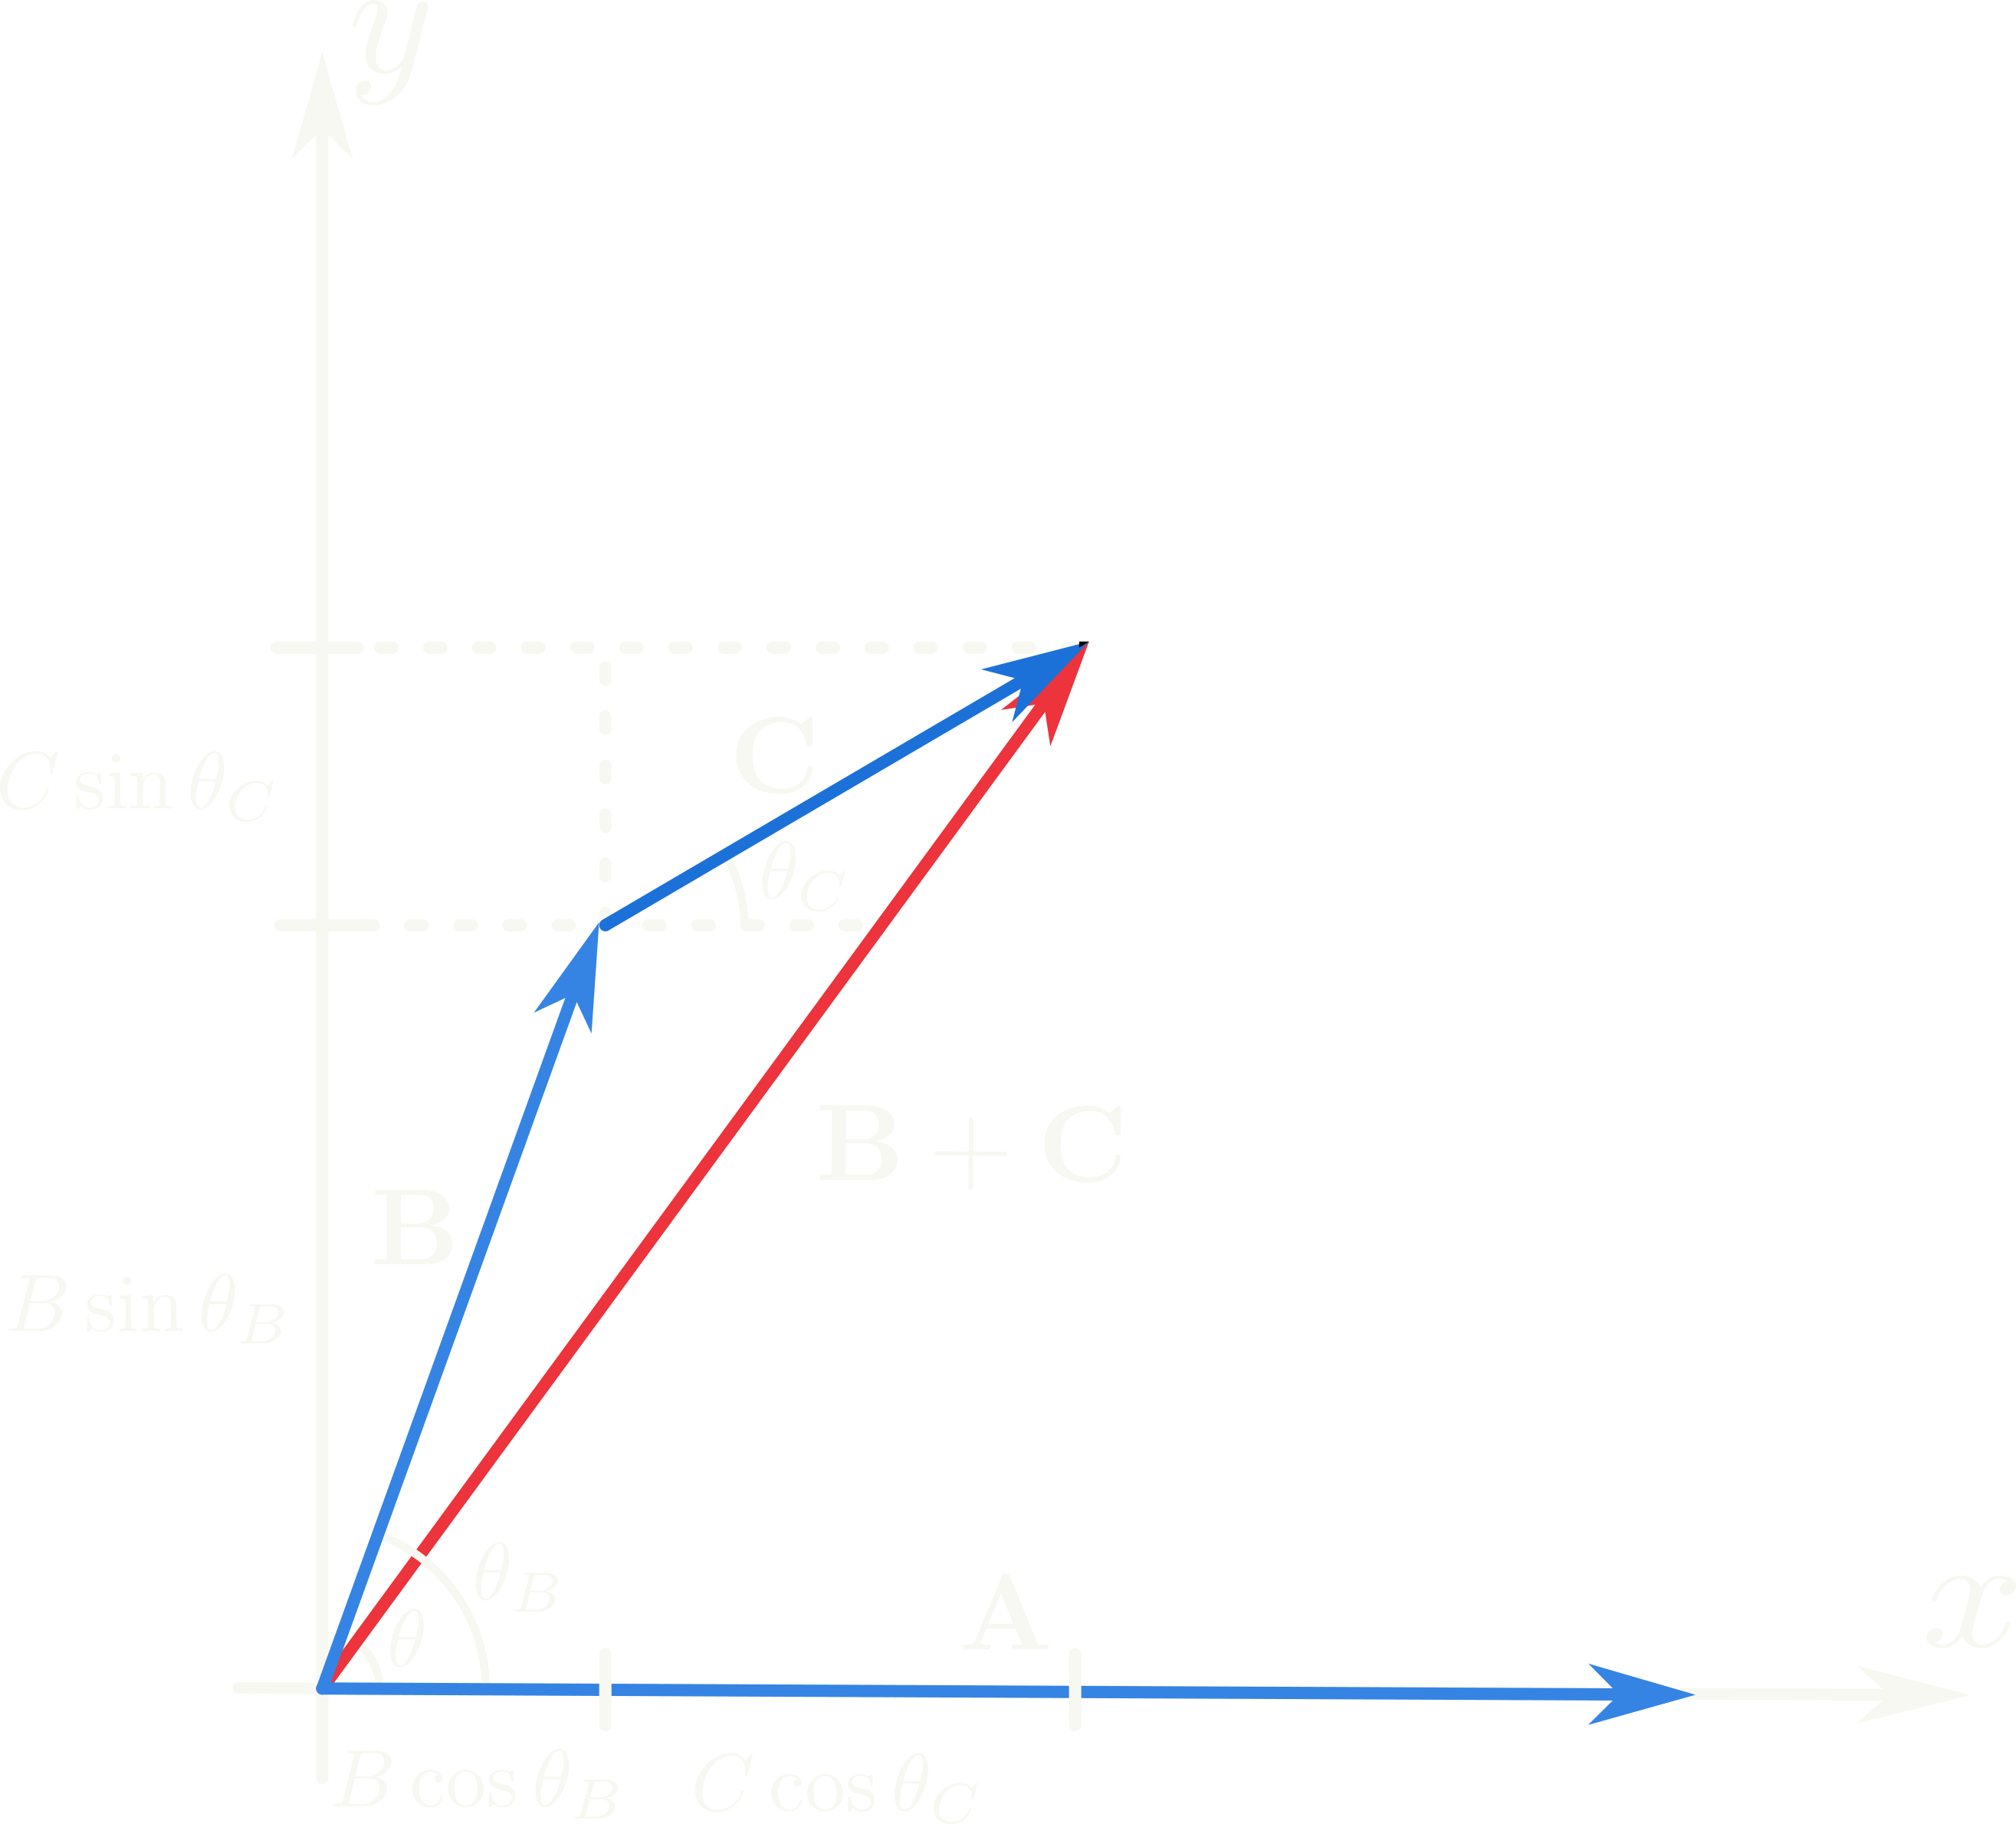
\includegraphics[width=0.5\linewidth]{images/fig1_1.png}
    \caption{Three Coplanar Vectors}
    \label{fig:1.1}
\end{figure}
(a) When three vectors are coplanar as shown in Figure \ref{fig:1.1}, the dot product is
\begin{align*}
    \vb{A} \cdot (\vb{B} + \vb{C}) &= \vb{A} \cdot \vb{B} + \vb{A} \cdot \vb{C} \\
    A (B+C) \cos \theta &= A B \cos \theta_B + A C \cos \theta_C
\end{align*}
Since $B \cos{\theta_B} + B \cos{\theta_C} = (B+C)\cos{\theta}$ from Figure \ref{fig:1.1}, the
distriubtive property holds true. The cross product also holds true since
$B \sin{\theta_B} + B \sin{\theta_C} = (B+C)\sin{\theta}$, and multiplying by $A$ on both sides
gives the same result as the distriubtive property:
\begin{align*}
    \vb{A} \cp (\vb{B} + \vb{C}) &= \vb{A} \cp\vb{B} + \vb{A} \cp\vb{C} \\
    A (B+C) \sin \theta &= A B \sin \theta_B + A C \sin \theta_C
\end{align*}

(b) In the general case in three-dimensional space, each vector has three components: \\
$\vb{A} = (A_x, A_y, A_z)$. Therefore,
\begin{align*}
    \vb{A} \cdot (\vb{B} + \vb{C}) &=
        \vb{A} \cdot (B_x + C_x, B_y + C_y, B_z + C_z) \\
    &= A_x (B_x + C_x) + A_y (B_y + C_y) + A_z (B_z + C_z) \\
    &= A_x B_x + A_y B_y + A_z B_z + A_x C_x + A_y C_y + A_z C_z \\
    &= \vb{A} \cdot \vb{B} + \vb{A} \cdot \vb{C}
\end{align*}

\paragraph{1.2}
Setting $\vb{A} = \vb{B} = (1, 1, 1)$ and $\vb{C} = (1, 1, -1)$:
\begin{align*}
    (\vb{A} \cp \vb{B}) \cp \vb{C} &\overset{?}{=} \vb{A} \cp (\vb{B} \cp \vb{C})\\
    0 &\overset{?}{=} (1, 1, 1) \cp [(1, 1, 1) \cp (1, 1, -1)]\\
    0 &\overset{?}{=} (1, 1, 1) \cp (-2, 2, 0)\\
    0 &\neq (-2, -2, 4)
\end{align*}
where the cross product of parallel vectors $\vb{A} \cp \vb{B} = 0$. Therefore, the cross product is
not associative.

\paragraph{1.3}
Taking the dot product of a unit cube's body diagonals $\vb{A} = (1, 1, 1)$, $\vb{B} = (1, 1, -1)$:
\begin{align*}
    \vb{A} \cdot \vb{B} &= AB \cos{\theta} \\
    1 &= 3 \cos{\theta} \\
    \theta &= \arccos{1/3} \approx \ang{70.53}
\end{align*} 

\paragraph{1.4}
The cross product of two vectors coplanar to the shaded plane---$\vb{A} = (-1, 2, 0)$,
$\vb{B} = (-1, 0, 3)$---is parallel to the normal unit vector $\vu{n}$ of the plane:
\begin{align*}
    \vb{A} \cp \vb{B} &= \vb{C} \\
    \begin{vmatrix}
        \vu{x} & \vu{y} & \vu{z} \\
        -1 & 2 & 0 \\
        -1 & 0 & 3
    \end{vmatrix} &= (6, 3, 2) \\
\end{align*}
where $\vu{n} = \vb{C} / C$, and $C = \sqrt{6^2 + 3^2 + 2^2} = \sqrt{49} = 7$. Therefore,
\begin{align*}
    \vu{n} &= \frac{1}{7} (6, 3, 2)
\end{align*}

\paragraph{1.5}
Proving the ``BAC--CAB'' rule for three-dimensional vectors:
\begin{align*}
    \vb{A} \cp (\vb{B} \cp \vb{C}) &= \vb{A} \cp
    \begin{vmatrix}
        \vu{x} & \vu{y} & \vu{z} \\
        B_x & B_y & B_z \\
        C_x & C_y & C_z
    \end{vmatrix} \\
    &= \begin{vmatrix}
        \vu{x} & \vu{y} & \vu{z} \\
        A_x & A_y & A_z \\
        B_y C_z - B_z C_y & B_z C_x - B_x C_z & B_x C_y - B_y C_x
    \end{vmatrix}
\end{align*}
where the $x$ component is $A_y (B_x C_y - B_y C_x) - A_z (B_z C_x - B_x C_z)$. Similarly,
\begin{align*}
    \vb{B}(\vb{A} \cdot \vb{C}) - \vb{C}(\vb{A} \cdot \vb{B}) &=
        \vb{B} (A_x C_x + A_y C_y + A_z C_z) - \vb{C} (A_x B_x + A_y B_y + A_z B_z)
\end{align*}
where $x$ component simplifes to
\begin{align*}
    B_x (\cancel{A_x C_x} + A_y C_y + A_z C_z) - C_x (\cancel{A_x B_x}+ A_y B_y + A_z B_z) &=
        A_y (B_x C_y - B_y C_x) - A_z (B_z C_x - B_x C_z)
\end{align*}
the same is done for the $y$ and $z$ components. Therefore, the ``BAC--CAB'' rule holds true.

\paragraph{1.6}
\begin{align*}
    [\vb{A} \cp (\vb{B} \cp \vb{C})] + [\vb{B} \cp (\vb{C} \cp \vb{A})] 
        + [\vb{C} \cp (\vb{A} \cp \vb{B})]
    &= \cancel{\vb{B}(\vb{A} \cdot \vb{C})} - \vb{C}(\vb{A} \cdot \vb{B})
    + \vb{C}(\vb{B} \cdot \vb{A}) = 0 \\ &- \vb{A}(\vb{B} \cdot \vb{C})
    + \vb{A}(\vb{C} \cdot \vb{B}) - \cancel{\vb{B}(\vb{C} \cdot \vb{A})}\\
\end{align*}
since dot product is associative, the first and last terms cancel out, and the middle terms also
cancel out with each other.

\begin{align*}
    \vb{A} \cp (\vb{B} \cp \vb{C}) &= (\vb{A} \cp \vb{B}) \cp \vb{C} \\
    \vb{B} (\vb{A} \cdot \vb{C}) - \vb{C} (\vb{A} \cdot \vb{B}) &=
    \vb{B} (\vb{A} \cdot \vb{C}) - \vb{A} (\vb{B} \cdot \vb{C}) \\
    0 &= -\vb{C} (\vb{A} \cdot \vb{B}) + \vb{A} (\vb{B} \cdot \vb{C}) \\
    0 &= -\vb{B} (\vb{C} \cp \vb{A}) = (\vb{C} \cp \vb{A}) \cp \vb{B}
\end{align*}
For the relation to hold true, either the vectors $\vb{A}$ and $\vb{C}$  are parallel
($\vb{A} \cp \vb{A} = 0$) or $\vb{B}$ is perpendicular to both $\vb{A}$ and $\vb{C}$
($\vb{A} \cdot \vb{B} = \vb{B} \cdot \vb{C} = 0$).

\paragraph{1.7}
Finding the seperation vector $\boldscriptr$:
\begin{align*}
    \boldscriptr &= \vb{r} - \vb{r}' = (4, 6, 8) - (2, 8, 7) = (2, -2, 1) \\
    \scriptr &= \sqrt{2^2 + (-2)^2 + 1^2} = 3 \\
    \vu{\boldscriptr} &= \quantity(\frac{2}{3}, -\frac{2}{3}, \frac{1}{3})
\end{align*}

\paragraph{1.8} (a)
\begin{align*}
    \begin{split}
        \bar{A}_y \bar{B}_y + \bar{A}_z \bar{B}_z =
        (A_y \cos{\phi} &+ A_z \sin{\phi})(B_y \cos{\phi} + B_z \sin{\phi}) \\
        &+ (-A_y \sin\phi + A_z \cos\phi)(-B_y \sin\phi + B_z \cos\phi)
    \end{split} \\
    \begin{split}
        = A_y B_y \cos^2\phi + A_z B_z \sin^2\phi
        &+ \cancel{A_y B_z \sin\phi\cos\phi} + \bcancel{A_z B_y \sin\phi\cos\phi} \\
        + A_y B_y \sin^2\phi &- \cancel{A_y B_z \sin\phi\cos\phi} 
        - \bcancel{A_z B_y \sin\phi\cos\phi} + A_z B_z \cos^2\phi
    \end{split} \\
    = A_y B_y (\sin^2\phi + \cos^2\phi) &+ A_z B_z (\sin^2\phi + \cos^2\phi) \\
    \bar{A}_y \bar{B}_y + \bar{A}_z \bar{B}_z &= A_y B_y + A_z B_z
\end{align*}
(b) To preserve length $\abs{\bar{A}} = \abs{A}$. Squaring both sides and expanding gives
\begin{align*}
    \bar{A}_x^2 + \bar{A}_y^2 + \bar{A}_z^2 = A_x^2 + A_y^2 + A_z^2
\end{align*}
in summation form,
\begin{align*}
    \sum_{i=1}^3 \bar{A}_i \bar{A}_i
    = \sum_{i=1}^3 \quantity(\sum_{j=1}^3 R_{ij} A_j) \quantity(\sum_{k=1}^3 R_{ik} A_k)
    = \sum_{i=1}^3 \sum_{j=1}^3 \sum_{k=1}^3 R_{ij} R_{ik} A_j A_k
\end{align*}
For the length to be preserved, the indices $j$ and $k$ must be equal. Therefore,
\begin{align*}
    R_{ij} R_{ik} = \delta_{jk}
\end{align*}
where $\delta_{ij}$ is the Kronecker delta. Thus the length is preserved if the rotation
matrix is orthogonal, i.e.
\begin{align*}
    R_{ij} R_{ik} = (R^T)_{ji} R_{ik} = \delta_{jk} \qor R^T R = I
\end{align*}

\paragraph{1.9}
\begin{figure}[ht]
    \centering
    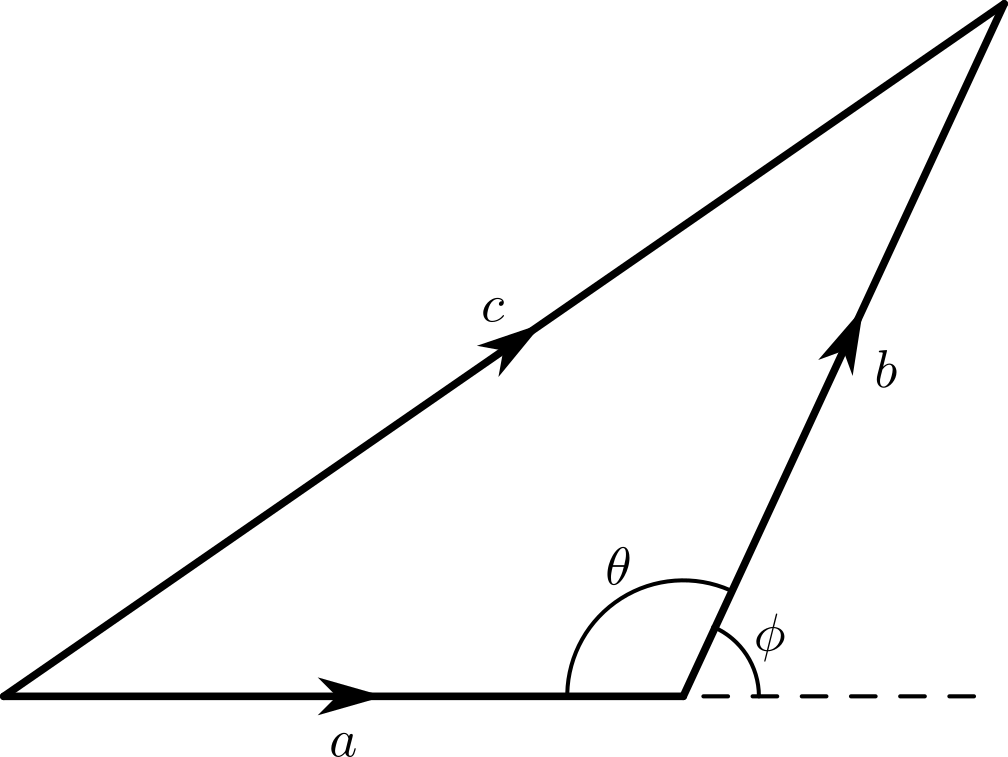
\includegraphics[width=0.4\linewidth]{images/fig1_9.png}
    \caption{Rotation of $\ang{120}$ about an axis through the origin and point $(1, 1, 1)$}
    \label{fig:1.9}
\end{figure}
From Figure \ref{fig:1.9}, the rotation is equivalent to changing the position of the basis vectors
$\vu{x} \to \vu{z}$, $\vu{y} \to \vu{x}$, and $\vu{z} \to \vu{y}$. Therefore, the rotation matrix is
a permutation matrix:
\begin{align*}
    R = \begin{pmatrix}
        0 & 0 & 1 \\
        1 & 0 & 0 \\
        0 & 1 & 0
    \end{pmatrix}
\end{align*}

\paragraph{1.10}
(a) Under a \textbf{translation} of coordinates $\bar{y} = y - a$, the origin $O$ and terminus
$A = (x, y, z)$ of some vector are translated to
\begin{align*}
    O \to O' &= (0, -a, 0)\\
    A \to A' &= (x, y - a, z)
\end{align*}
therefore, the translated vector is
\begin{align*}
    \overline{O'A'} &= (x, y - a, z) - (0, -a, 0) = (x, y, z) = \overline{OA} = \vb{A}
\end{align*}
which is the same as the original vector, so
\begin{align*}
    \mqty(\bar{A}_x \\ \bar{A}_y \\ \bar{A}_z) &=  \mqty(A_x \\ A_y \\ A_z)
\end{align*}

(b) Under \textbf{inversion} of coordinates, only the terminus changes
\begin{align*}
    O \to O' &= (0, 0, 0) \\
    A \to A' &= (-x, -y, -z)
\end{align*}
therefore, the inverted vector is
\begin{align*}
    \overline{O'A'} = (-x, -y, -z) \qor \mqty(\bar{A}_x \\ \bar{A}_y \\ \bar{A}_z) &=
        \mqty(-A_x \\ -A_y \\ -A_z)
\end{align*}

(c) The components of cross product under inversion
\begin{align*}
    \bar{\vb{A}} \cross \bar{\vb{B}} &= 
    \begin{pmatrix}
        \bar{A}_y \bar{B}_z - \bar{A}_z \bar{B}_y \\
        \bar{A}_z \bar{B}_x - \bar{A}_x \bar{B}_z \\
        \bar{A}_x \bar{B}_y - \bar{A}_y \bar{B}_x
    \end{pmatrix}
    =
    \begin{pmatrix}
        A_y B_z - A_z B_y \\
        A_z B_x - A_x B_z \\
        A_x B_y - A_y B_x
    \end{pmatrix}
\end{align*}
which is the same as the original cross product $\vb{A} \cross \vb{B}$. The cross product of two
pseudovectors is also a pseudovector. Torque $\vb{\tau} = \vb{r} \cross \vb{F}$ and magnetic force
$\vb{F} = q \vb{v} \cross \vb{B}$ are examples of pseudovectors.

(d) Scalar triple product under inversion
\begin{align*}
    \bar{A} \cdot (\bar{B} \cross \bar{C}) &= -\vb{A} \cdot (-\vb{B} \cross -\vb{C}) \\
    &= -\vb{A} \cdot (\vb{B} \cross \vb{C})
\end{align*}
the scalar triple product changes sign under inversion.

\paragraph{1.11}
(a) Finding gradient of $f(x, y, z) = x^2 + y^3 + z^4$:
\begin{align*}
    \grad{f} &= \pdv{f}{x} \vu{x} + \pdv{f}{y} \vu{y} + \pdv{f}{z} \vu{z} \\
    &= 2x \vu{x} + 3y^2 \vu{y} + 4z^3 \vu{z}
\end{align*}
(b) Gradient of $f(x, y, z) = x^2y^3z^4$:
\begin{align*}
    \grad{f} = 2xy^3z^4 \vu{x} + 3x^2y^2z^4 \vu{y} + 4x^2y^3z^3 \vu{z}
\end{align*}
(c) Gradient of $f(x, y, z) = e^x \sin(y) \ln(z)$:
\begin{align*}
    \grad{f} = e^x \vu{x} + e^x \cos(y) \ln(z) \vu{y} + \frac{e^x \sin(y)}{z} \vu{z}
\end{align*}

\paragraph{1.12}
The height of the hill (in feet) is given by the function
\begin{align*}
    h(x, y) = 10 (2xy - 3x^2 - 4y^2 - 18x + 28y + 12)
\end{align*}
where $y$ is north and $x$ is east in miles. The gradient of $h$ is
\begin{align*}
    \grad{h} &= 10 (2y - 6x - 18) \vu{x} + 10 (2x - 8y + 28) \vu{y}
\end{align*}
(a) The top of the hill is a stationary point, so the summit is found by setting the gradient to
zero which gives the system of equations
\begin{align*}
    0 &= 2y - 6x - 18 & 0 &= 2x - 8y + 28
\end{align*}
adding the first equation to 3 times the second equation gives
\begin{align*}
    0 &= 2y - 6x - 18 + 3(2x - 8y + 28) \\
    0 &= -22y + 66 \\
    y &= 3
\end{align*}
substituting $y = 3$ into the first equation
\begin{align*}
    0 = 2(3) - 6x - 18 \to x = -2
\end{align*}
Therefore, the top of the hill is at $(-2, 3)$ or 2 miles west and 3 miles north of the origin.

(b) The height of the hill is simply $h(-2, 3) = 10(12) = 720$ feet.

(c) The steepness of the hill at $h(1,1)$ is given by the magnitude of the gradient
\begin{align*}
    \abs{\grad{h}} &= 10\sqrt{(2y - 6x - 18)^2 + (2x - 8y + 28)^2} \\
    &= 10\sqrt{(2 - 6 - 18)^2 + (2 - 8 + 28)^2} \\
    &= 10\sqrt{(-22)^2 + (22)^2} = 220 \sqrt{2} \approx \qty{311}{ft/mi}
\end{align*}
The direction of the steepest slope is given by the vector in the direction of the gradient
at the point $\grad{h(1,1)} = 220(-\vb{x} + \vb{y})$, or simply northwest.

\paragraph{1.13}
Given the seperation vector
\begin{align*}
    \boldscriptr = (x - x') \vu{x} + (y - y') \vu{y} + (z - z') \vu{z} \qand 
    \scriptr = \sqrt{(x - x')^2 + (y - y')^2 + (z - z')^2}
\end{align*}
(a) Show that $\grad(\scriptr^2) = 2 \boldscriptr$:
\begin{align*}
    \grad(\scriptr^2) = 2(x - x') \vu{x} + 2(y - y') \vu{y} + 2(z - z') \vu{z} = 2 \boldscriptr
\end{align*}

(b)
\begin{align*}
    \grad(\frac{1}{\scriptr}) &= \pdv{x}(\frac{1}{\scriptr}) \vu{x}
        + \pdv{y}(\frac{1}{\scriptr}) \vu{y} + \pdv{z}(\frac{1}{\scriptr}) \vu{z} \\
\end{align*}
looking at the $x$ component,
\begin{align*}
    \pdv{x}(\frac{1}{\scriptr}) &= -\frac{1}{\scriptr^2} \pdv{x}(\scriptr) \\
    &= -\frac{1}{\scriptr^2} \pdv{x}(\sqrt{(x - x')^2 + (y - y')^2 + (z - z')^2}) \\
    &= -\frac{1}{\scriptr^2} \frac{1}{2}
        \frac{2(x - x')}{\sqrt{(x - x')^2 + (y - y')^2 + (z - z')^2}} \\
    &= -\frac{x - x'}{\scriptr^3}
\end{align*}
therefore,
\begin{align*}
    \grad(\frac{1}{\scriptr}) = -\frac{1}{\scriptr^3}
        [(x - x') \vu{x} + (y - y') \vu{y} + (z - z') \vu{z}]
    = -\frac{\boldscriptr}{\scriptr^3} 
    = -\frac{\vu{\boldscriptr}}{\scriptr^2}
\end{align*}

(c) The general formula is
\begin{align*}
    \grad(\scriptr^n) = n \scriptr^{n-1} \vu{\boldscriptr}
\end{align*}

\paragraph{1.14}
Given the rotation matrix
\begin{align*}
    \mqty(\bar{y} \\ \bar{z}) &= \mqty(\cos\phi & \sin\phi \\ -\sin\phi & \cos\phi)
    \mqty(y \\ z)
\end{align*}
or the two equations
\begin{align*}
    \bar{y} &= y \cos\phi + z \sin\phi \\
    \bar{z} &= -y \sin\phi + z \cos\phi
\end{align*}
differentiating with respect to $\bar{y}$ and $\bar{z}$ respectively gives
\begin{align*}
    1 &= \pdv{y}{\bar{y}}\cos\phi + \pdv{z}{\bar{y}}\sin\phi \\
    1 &= -\pdv{y}{\bar{z}}\sin\phi + \pdv{z}{\bar{z}}\cos\phi
\end{align*}
this can only be true if
\begin{align*}
    \pdv{y}{\bar{y}} = \cos\phi     ,\quad      \pdv{z}{\bar{y}} = \sin\phi
    \qand \pdv{y}{\bar{z}} = -\sin\phi      ,       \pdv{z}{\bar{z}} = \cos\phi
\end{align*}
which satisfies the trig identity $\sin^2\phi + \cos^2\phi = 1$. Differentiating $f$ with respect to
the rotated coordinates $\bar{y}$ and $\bar{z}$ is given by
\begin{align*}
    \pdv{f}{\bar{y}} &= \pdv{f}{y} \pdv{y}{\bar{y}} + \pdv{f}{z} \pdv{z}{\bar{y}}
    = \pdv{f}{y} \cos\phi + \pdv{f}{z} \sin\phi \\
    \pdv{f}{\bar{z}} &= \pdv{f}{y} \pdv{y}{\bar{z}} + \pdv{f}{z} \pdv{z}{\bar{z}}
    = -\pdv{f}{y} \sin\phi + \pdv{f}{z} \cos\phi
\end{align*}
therefore, the gradient of $f$ transforms as a vector under rotations given by
\begin{align*}
    \overline{\grad{f}} = \pdv{f}{\bar{y}} \vu{\bar{y}} + \pdv{f}{\bar{z}} \vu{\bar{z}}
    = \quantity(\pdv{f}{y} \cos\phi + \pdv{f}{z} \sin\phi) \vu{\bar{y}}
    + \quantity(-\pdv{f}{y} \sin\phi + \pdv{f}{z} \cos\phi) \vu{\bar{z}}
\end{align*}
or in matrix form
\begin{align*}
    \overline{\grad{f}} = \mqty(\cos\phi & -\sin\phi \\ \sin\phi & \cos\phi) \grad{f}
\end{align*}
where the gradient is a column vector
\begin{align*}
    \grad{f} = \begin{pmatrix}
        \pdv{f}{y} \\[1ex] \pdv{f}{z}
    \end{pmatrix}
\end{align*}

\paragraph{1.15}
(a) Calculating divergence of $v_a = x^2\vu{x} + 3xz^2\vu{y} - 2xz\vu{z}$:
\begin{align*}
    \div{v_a} &= \pdv{v_{ax}}{x} + \pdv{v_{ay}}{y} + \pdv{v_{az}}{z} \\
    &= 2x + 0 - 2x = 0
\end{align*}

(b) $v_b = xy\vu{x} + 2yz\vu{y} + 3zx\vu{z}$:
\begin{align*}
    \div{v_b} &= y + 2z + 3x
\end{align*}

(c) $v_c = y^2\vu{x} + (2xy + z^2)\vu{y} + 2yz\vu{z}$:
\begin{align*}
    \div{v_c} &= 0 + 2x + 2y = 2(x + y)
\end{align*}

\paragraph{1.16}
\begin{figure}[ht]
    \centering
    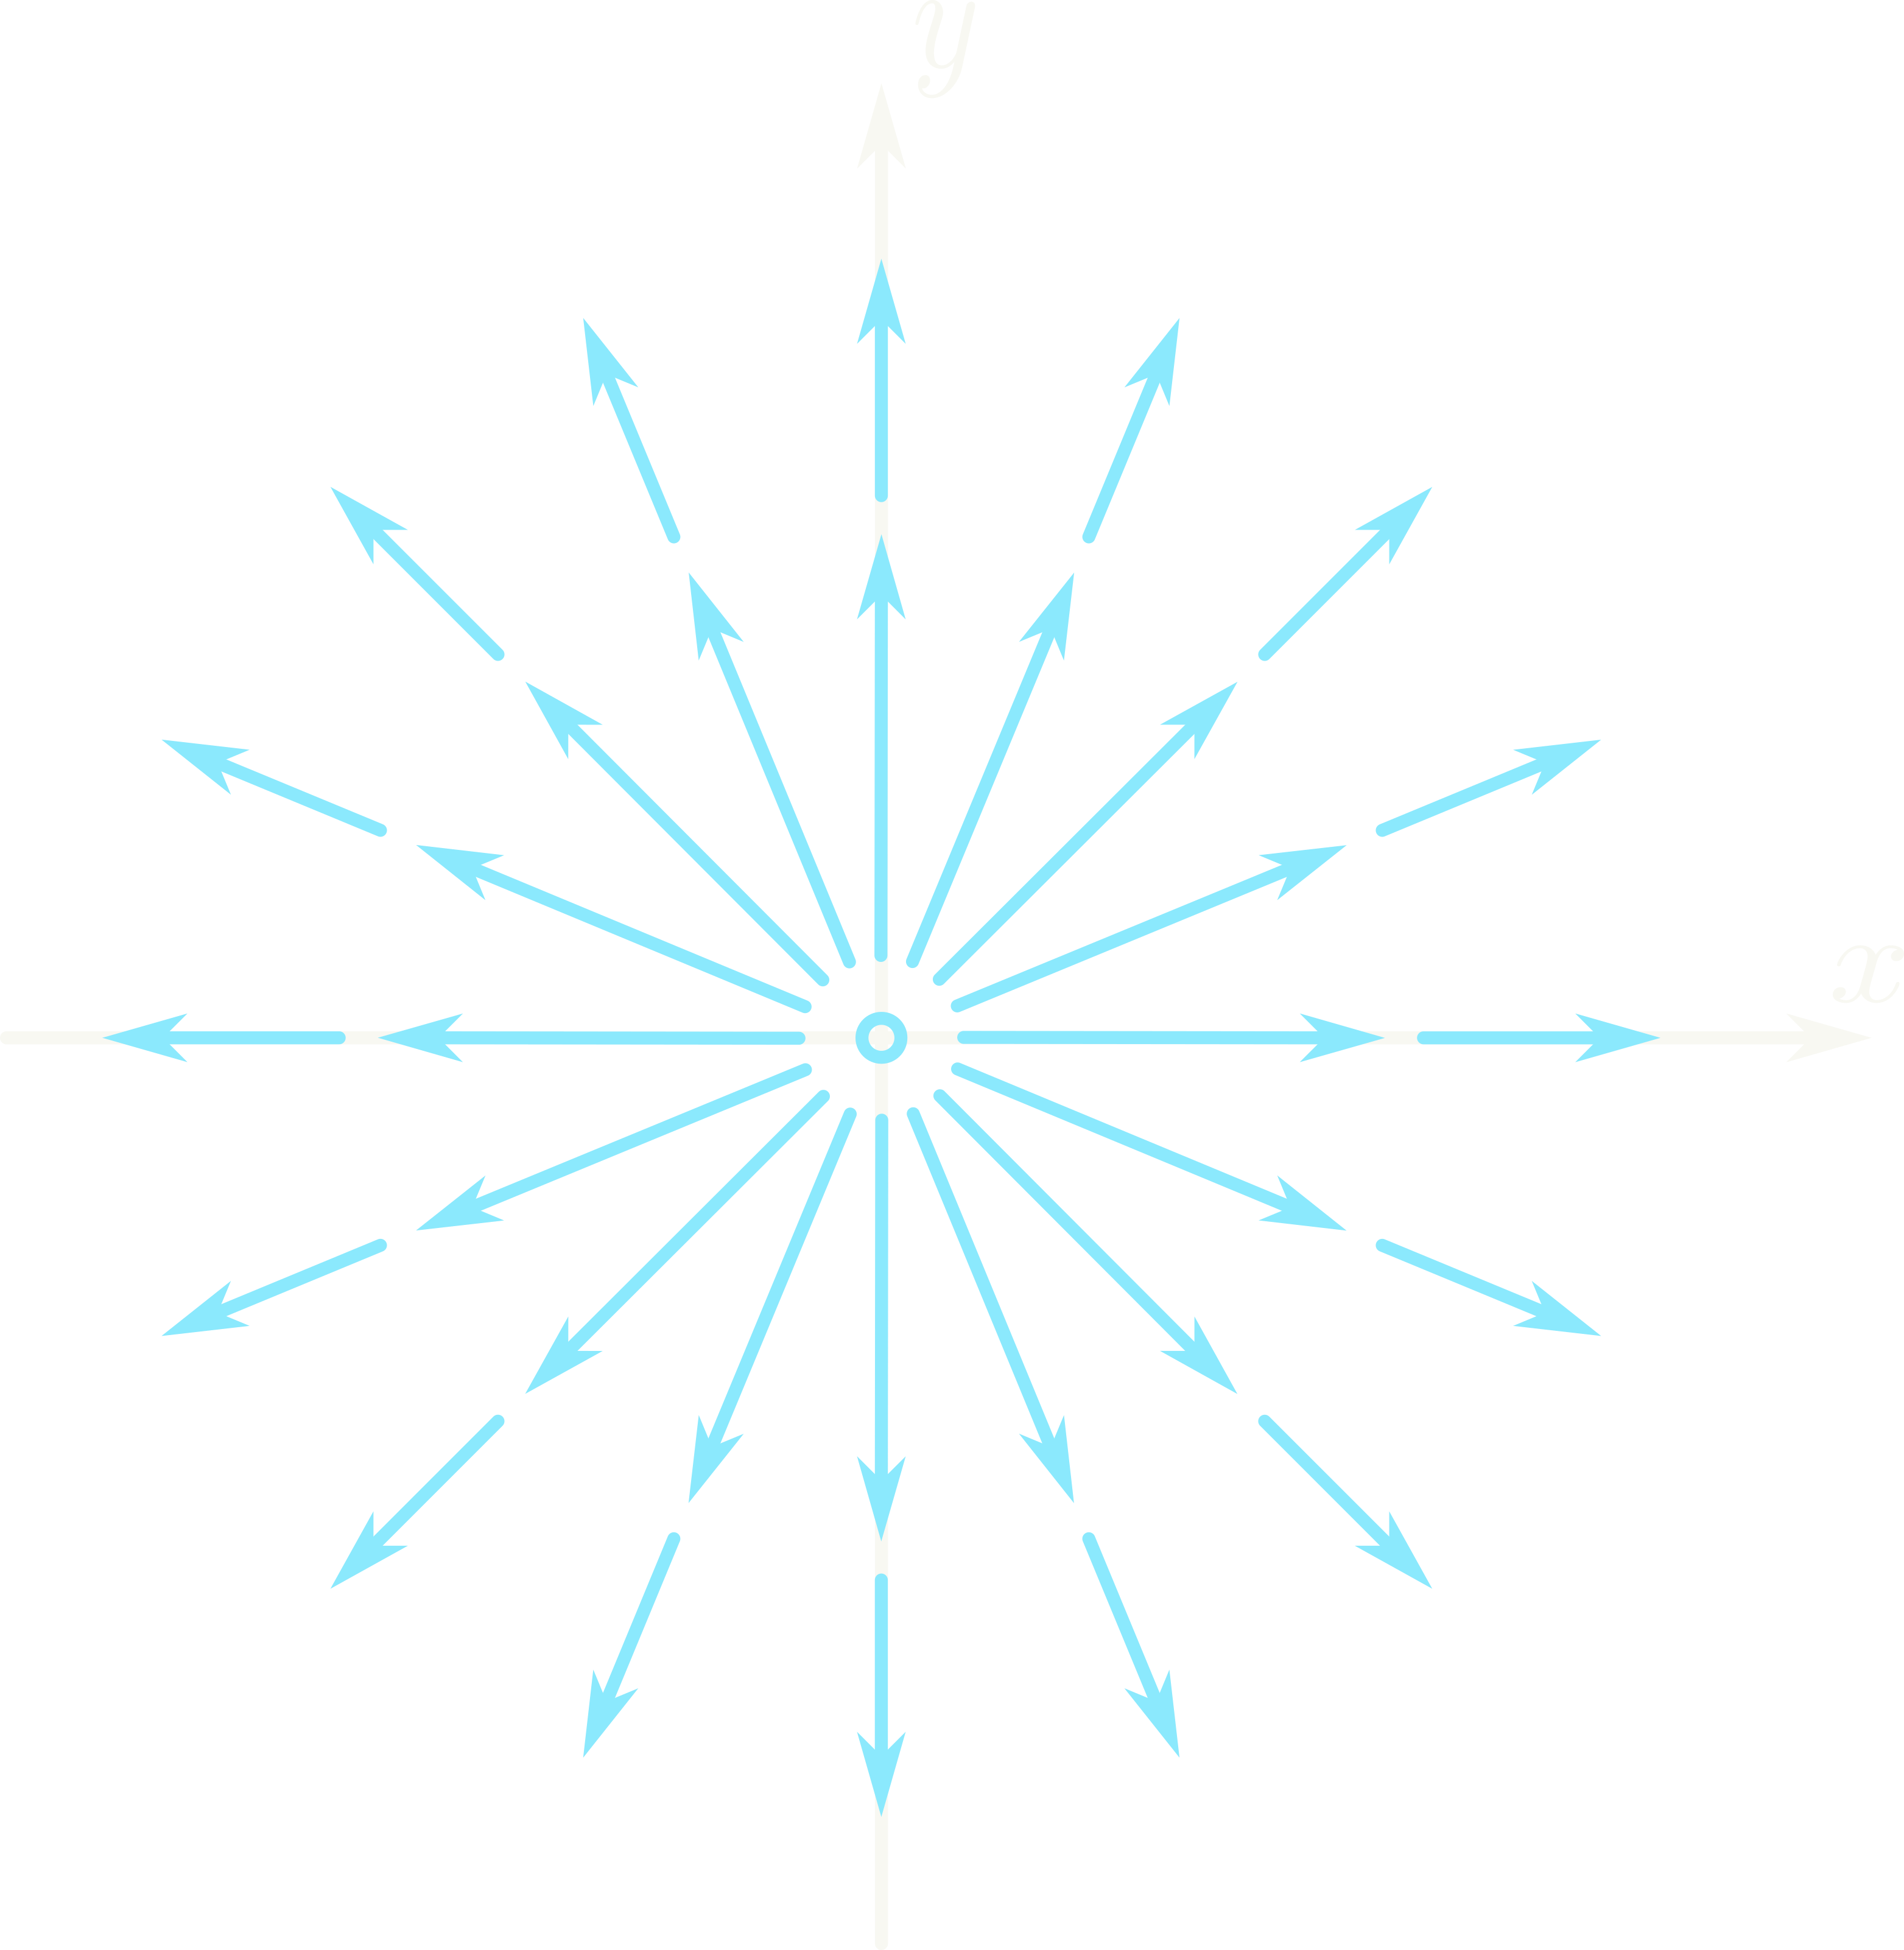
\includegraphics[width=0.4\linewidth]{images/fig1_16.png}
    \caption{Sketch of the vector field $\vb{v} = \vu{r} / r^2$}
    \label{fig:1.16}
\end{figure}
Given
\begin{align*}
    r = \sqrt{x^2 + y^2 + z^2} \qand
    \vu{r} = \frac{\vb{r}}{r} = \frac{x\vu{x} + y\vu{y} + z\vu{z}}{\sqrt{x^2 + y^2 + z^2}}
\end{align*}
where $\vb{r} = x\vu{x} + y\vu{y} + z\vu{z}$ is the position vector. The vector functions is
\begin{align*}
    v = \frac{\vu{r}}{r^2} = \frac{\vb{r}}{r^3}
\end{align*}
where the components are
\begin{align*}
    v_x = \frac{x}{r^3} \qand v_y = \frac{y}{r^3} \qand v_z = \frac{z}{r^3}
\end{align*}
Looking at the $x$ component of the divergence,
\begin{align*}
    [\div{\vb{v}}]_x &= \pdv{v_x}{x} \\
    &= \pdv{x}(\frac{x}{r^3}) \\
    &= \pdv{x}(\frac{x}{(x^2 + y^2 + z^2)^{3/2}}) \qq{using chain rule...}\\
    &= \frac{1}{(x^2 + y^2 + z^2)^{3/2}} - \frac{3x^2}{(x^2 + y^2 + z^2)^{5/2}} \\
    &= \frac{1}{r^3} - \frac{3x^2}{r^5}
\end{align*}
therefore, the divergence of $\vb{v}$ is
\begin{align*}
    \div{\vb{v}} &= \quantity(\frac{1}{r^3} - \frac{3x^2}{r^5})
        + \quantity(\frac{1}{r^3} - \frac{3y^2}{r^5})
        + \quantity(\frac{1}{r^3} - \frac{3z^2}{r^5}) \\
    &= \frac{3}{r^3} - 3\frac{x^2 + y^2 + z^2}{r^5} \\
    &= \frac{3}{r^3} - 3\frac{r^2}{r^5} = 0
\end{align*}
This is consistent with the sketch in Figure \ref{fig:1.16} because the vector field is not 
`sourcing' or `sinking'.

\paragraph{1.17}
Given
\begin{align*}
    \bar{v}_y = v_y \cos\phi + v_z \sin\phi \qand \bar{v}_z = -v_y \sin\phi + v_z \cos\phi
\end{align*}
Calculating the derivatives
\begin{align*}
    \pdv{\bar{v}_y}{\bar{y}} &= \pdv{v_y}{\bar{y}} \cos\phi + \pdv{v_z}{\bar{y}} \sin\phi \\
    \pdv{\bar{v}_z}{\bar{z}} &= -\pdv{v_y}{\bar{z}} \sin\phi + \pdv{v_z}{\bar{z}} \cos\phi
\end{align*}
from Problem 1.14,
\begin{align*}
    \pdv{f}{\bar{y}} &= \pdv{f}{y} \cos\phi + \pdv{f}{z} \sin\phi \\
    \pdv{f}{\bar{z}} &= -\pdv{f}{y} \sin\phi + \pdv{f}{z} \cos\phi
\end{align*}
therefore, the derivatives are rewritten as
\begin{align*}
    \pdv{\bar{v}_y}{\bar{y}} &=
        \quantity(\pdv{v_y}{y} \pdv{y}{\bar{y}} + \pdv{v_y}{z} \pdv{z}{\bar{y}}) \cos\phi 
        + \quantity(\pdv{v_z}{y} \pdv{y}{\bar{z}} + \pdv{v_z}{y} \pdv{z}{\bar{z}}) \sin\phi \\
    &= \quantity(\pdv{v_y}{y} \cos\phi + \pdv{v_y}{z} \sin\phi) \cos\phi 
        + \quantity(\pdv{v_z}{y} \cos\phi + \pdv{v_z}{z} \sin\phi) \sin\phi
\end{align*}
and likewise,
\begin{align*}
    \pdv{\bar{v}_z}{\bar{z}} &=
        - \quantity(-\pdv{v_y}{y} \sin\phi +\pdv{v_y}{z} \cos\phi) \sin\phi 
        + \quantity(-\pdv{v_z}{y} \sin\phi + \pdv{v_z}{z} \cos\phi) \cos\phi \\
\end{align*}
Finally adding the two equations together gives
\begin{align*}
    \div{\bar{\vb{v}}} &= \pdv{\bar{v}_y}{\bar{y}} + \pdv{\bar{v}_z}{\bar{z}} \\
    &= \pdv{v_y}{y} \cos^2\phi + \pdv{v_y}{z} \sin\phi\cos\phi 
        + \pdv{v_z}{y} \sin\phi\cos\phi + \pdv{v_z}{z} \sin\phi^2 \\
    &+ \pdv{v_y}{y} \sin^2\phi - \pdv{v_y}{z} \sin\phi\cos\phi
        - \pdv{v_z}{y} \sin\phi\cos\phi + \pdv{v_z}{z} \cos^2\phi \\
    &= (\sin\phi^2 + \cos\phi^2)\quantity[\pdv{v_y}{y} + \pdv{v_z}{z}] \\
    &= \pdv{v_y}{y} + \pdv{v_z}{z}
\end{align*}
which shows that the divergence transforms as a scalar under rotations.

\paragraph{1.18}
Curl of vector functions from Problem 1.15:
(a) $\vb{v}_a = x^2\vu{x} + 3xz^2\vu{y} - 2xz\vu{z}$:
\begin{align*}
    \curl{\vb{v}_a} &= \mqty|
        \vu{x} & \vu{y} & \vu{z} \\
        \pdv{x} & \pdv{y} & \pdv{z} \\
        x^2 & 3xz^2 & -2xz
    | \\
    &= \vu{x} (0 - 6xz) - \vu{y} (-2z - 0) + \vu{z} (3z^2 - 0) \\
    &= -6xz\vu{x} + 2z\vu{y} + 3z^2\vu{z}
\end{align*}

(b) $\vb{v}_b = xy\vu{x} + 2yz\vu{y} + 3zx\vu{z}$:
\begin{align*}
    \curl{\vb{v}_b} &= \begin{vmatrix}
        \vu{x} & \vu{y} & \vu{z} \\
        \pdv{x} & \pdv{y} & \pdv{z} \\
        xy & 2yz & 3zx
    \end{vmatrix} \\
    &= \vu{x} (0 - 2y) - \vu{y} (3z - 0) + \vu{z} (0 - x) \\
    &= -2y\vu{x} - 3z\vu{y} - x\vu{z}
\end{align*}

(c) $\vb{v}_c = y^2\vu{x} + (2xy + z^2)\vu{y} + 2yz\vu{z}$:
\begin{align*}
    \curl{\vb{v}_c} &= \begin{vmatrix}
        \vu{x} & \vu{y} & \vu{z} \\
        \pdv{x} & \pdv{y} & \pdv{z} \\
        y^2 & 2xy + z^2 & 2yz
    \end{vmatrix} \\
    &= \vu{x} (2z - 2z) - \vu{y} (0 - 0) + \vu{z} (2y - 2y) \\
    &= 0
\end{align*}

\paragraph{1.19}
\begin{figure}[ht]
    \centering
    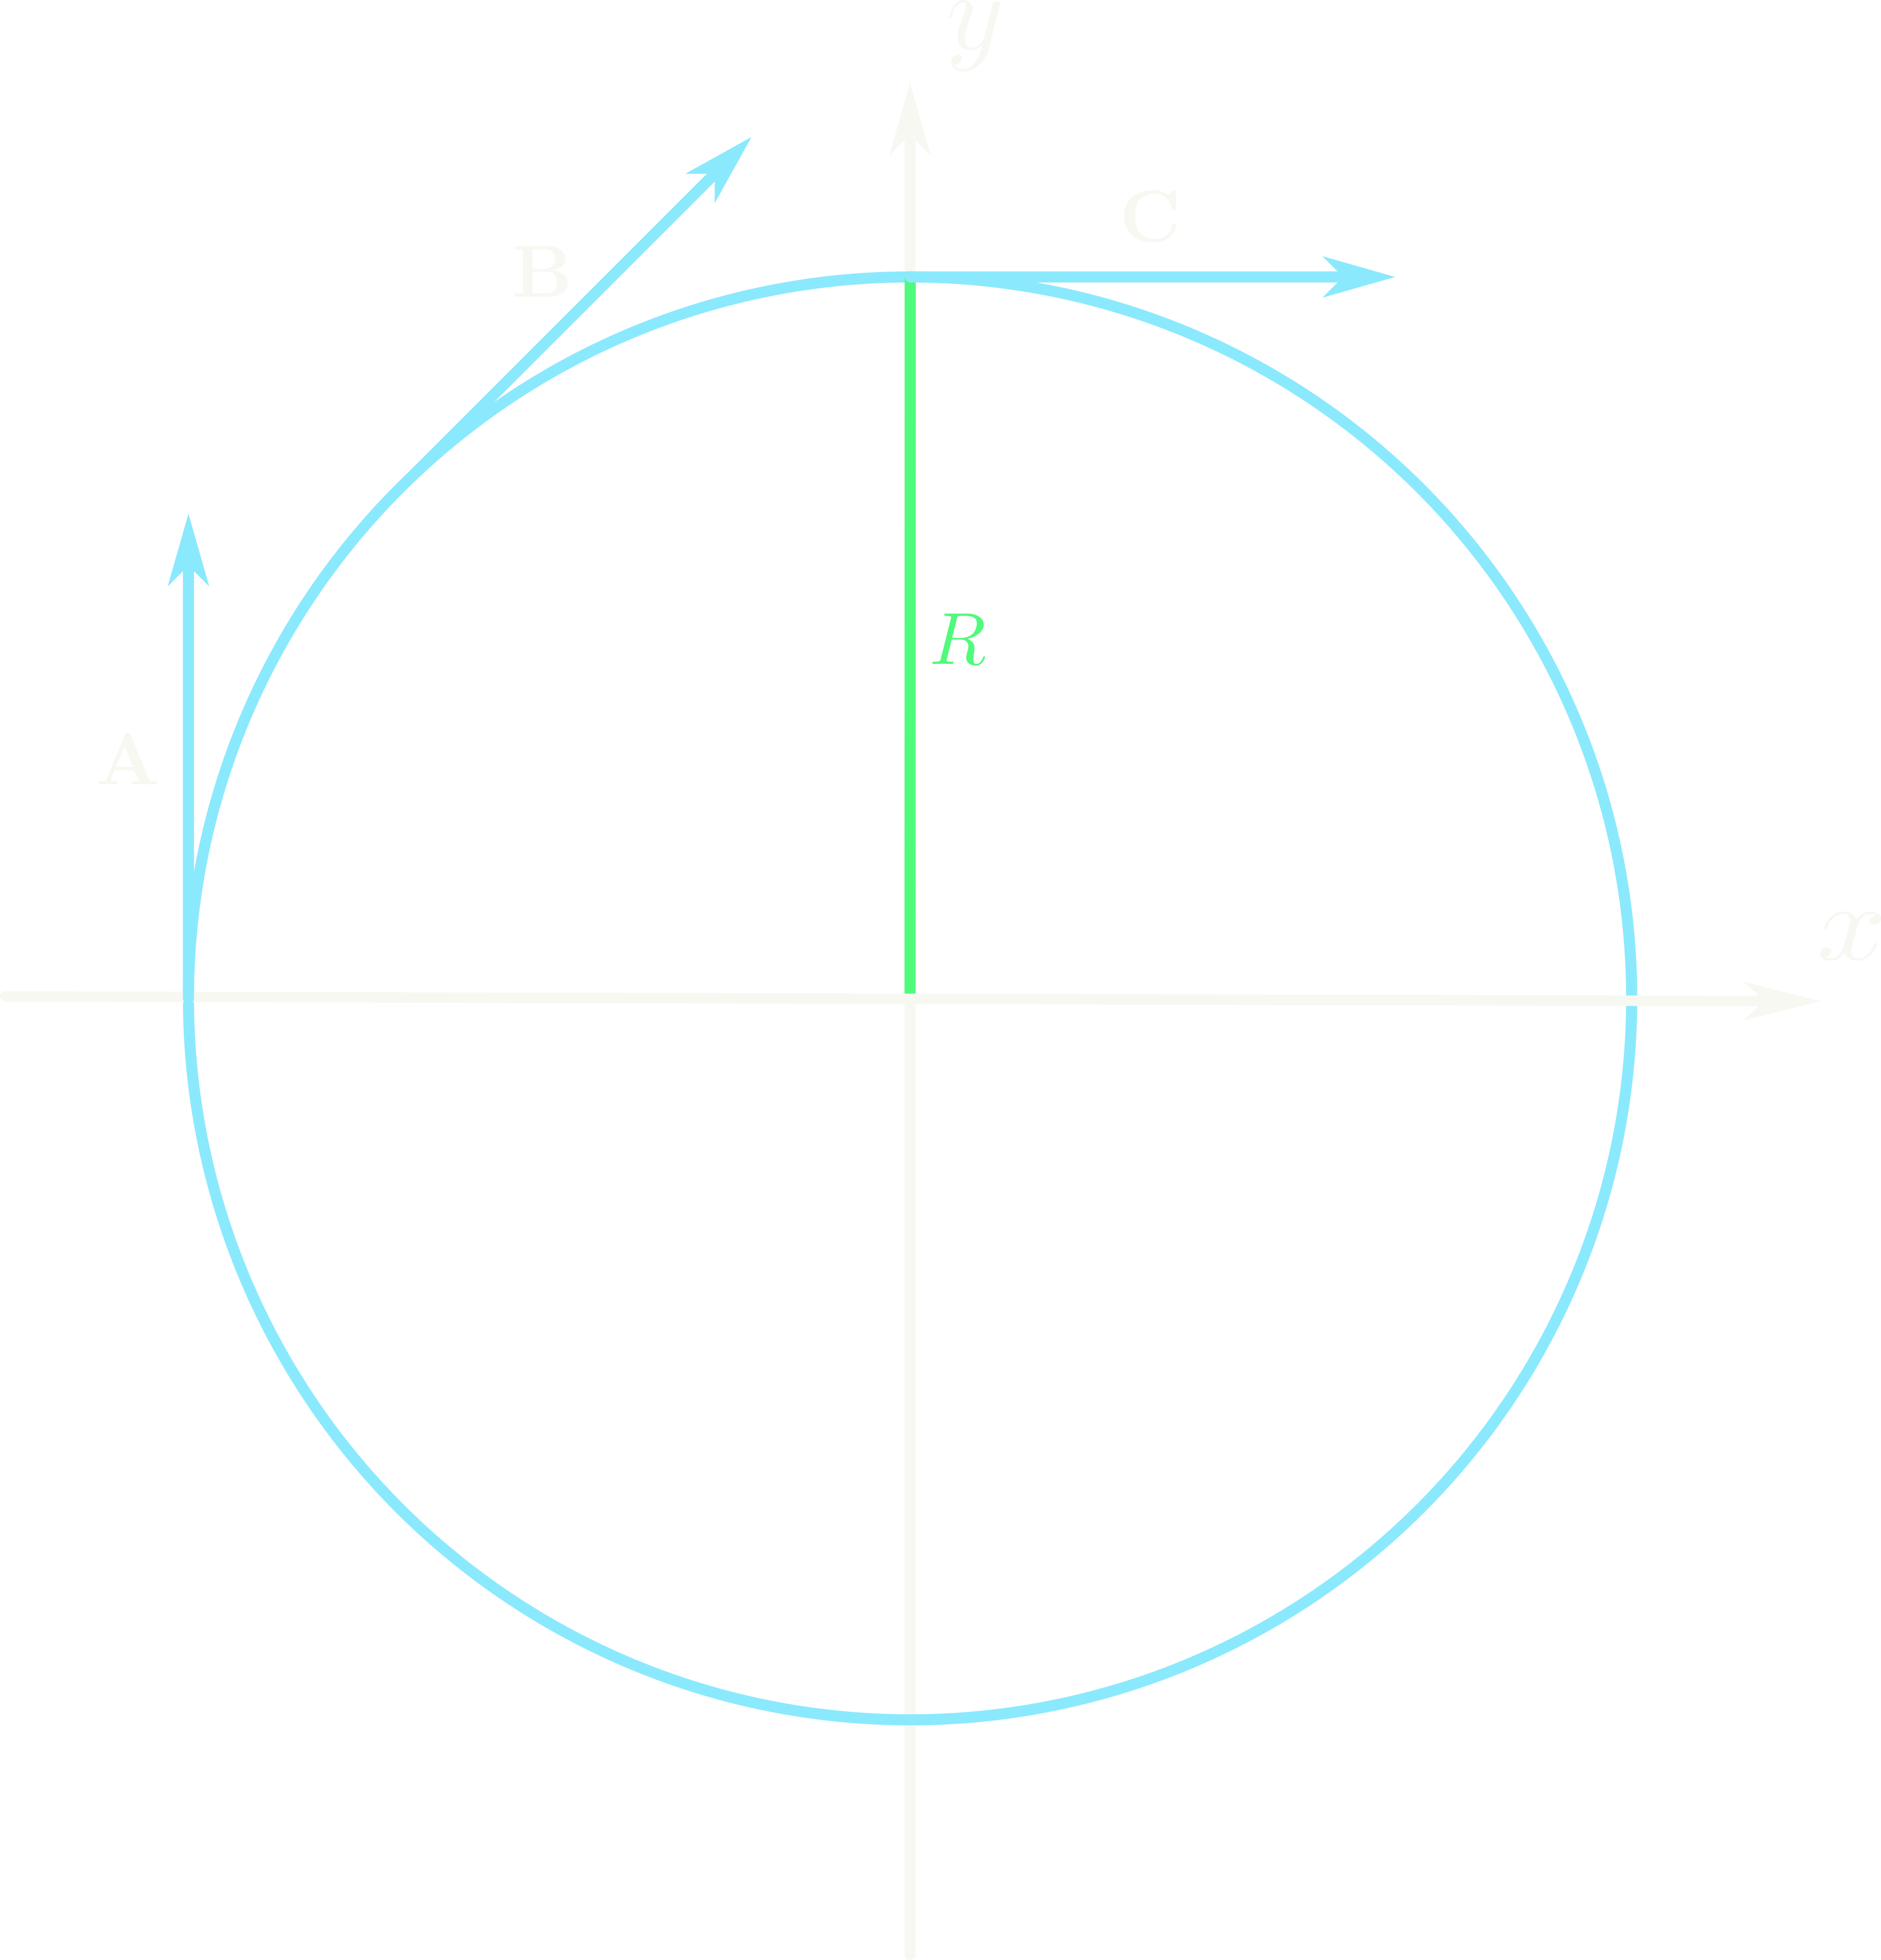
\includegraphics[width=0.4\linewidth]{images/fig1_19.png}
    \caption{Sketch of the vector field pointing clockwise around a circle of radius $R$}
    \label{fig:1.19}
\end{figure}
From Figure \ref{fig:1.19}, the sign of $\pdv*{v_x}{y}$ is positive, and the sign of $\pdv*{v_y}{x}$
is negative. Therefore, the curl
\begin{align*}
    \curl{\vb{v}} = \vu{z} \quantity(\pdv{v_x}{y} - \pdv{v_y}{z}) 
\end{align*}
is in the negative $z$ direction, or into the page. This is consistent with the right-hand rule as
the thumb points into the page.

\paragraph{1.20}
Proof that the vector function
\begin{align*}
    \vb{g} = \frac{\vu{r}}{r^2} = \frac{\vb{r}}{r^3} = \frac{x\vu{x} + y\vu{y} + z\vu{z}}{r^3}
\end{align*}
has zero divergence and curl given
\begin{align*}
    \pdv{r}{x_i} = \frac{x_i}{r} \qand \pdv{x}{y} = \frac{y}{x} = 0
\end{align*}
From Problem 1.16, the divergence of $\vb{g}$ is
\begin{align*}
    \div{\vb{g}} &= \pdv{g_x}{x} + \pdv{g_y}{y} + \pdv{g_z}{z} \\
    &= \pdv{x}(\frac{x}{r^3}) + \pdv{y}(\frac{y}{r^3}) + \pdv{z}(\frac{z}{r^3}) \\
    &= \frac{1}{r^3} - \frac{3x^2}{r^5} + \frac{1}{r^3} - \frac{3y^2}{r^5}
        + \frac{1}{r^3} - \frac{3z^2}{r^5} \\
    &= \frac{3}{r^3} - \frac{3}{r^3} = 0
\end{align*}
and the curl is
\begin{align*}
    \curl{\vb{g}} &= \begin{vmatrix}
        \vu{x} & \vu{y} & \vu{z} \\
        \pdv{x} & \pdv{y} & \pdv{z} \\
        \frac{x}{r^3} & \frac{y}{r^3} & \frac{z}{r^3}
    \end{vmatrix} \\
    &= \vu{x} (0 - 0) - \vu{y} (0 - 0) + \vu{z} (0 - 0) = 0
\end{align*}

\paragraph{1.21}
Proving product rule for (i)
\begin{align*}
    \grad(fg) &= \pdv{(fg)}{x} \vu{x} + \pdv{(fg)}{y} \vu{y} + \pdv{(fg)}{z} \vu{z} \\
    &= \quantity(\pdv{f}{x} g + f \pdv{g}{x}) \vu{x} + \quantity(\pdv{f}{y} g + f \pdv{g}{y}) \vu{y}
        + \quantity(\pdv{f}{z} g + f \pdv{g}{z})  \vu{z}\\
    &= f\quantity(\pdv{g}{x} + \pdv{g}{y} + \pdv{g}{z})
        + g\quantity(\pdv{f}{x} + \pdv{f}{y} + \pdv{f}{z}) \\
    &= f\grad{g} + g\grad{f}
\end{align*}
(iv)
\begin{align*}
    \div(\vb{A} \cp \vb{B}) &= \div \begin{vmatrix}
        \vu{x} & \vu{y} & \vu{z} \\
        A_x & A_y & A_z \\
        B_x & B_y & B_z
    \end{vmatrix} \\
    &= \div [(A_y B_z - A_z B_y) \vu{x} + (A_z B_x - A_x B_z) \vu{y}
        + (A_x B_y - A_y B_x) \vu{z}] \\
    &= \pdv{x}(A_y B_z - A_z B_y) + \pdv{y}(A_z B_x - A_x B_z) + \pdv{z}(A_x B_y - A_y B_x) \\
    &= \qt(\pdv{A_y}{x} B_z + A_y \pdv{B_z}{x} - \pdv{A_z}{x} B_y - A_z \pdv{B_y}{x}) 
    + \qt(\pdv{A_z}{y} B_x + A_z \pdv{B_x}{y} - \pdv{A_x}{y} B_z - A_x \pdv{B_z}{y}) \\
    &+ \qt(\pdv{A_x}{z} B_y + A_x \pdv{B_y}{z} - \pdv{A_y}{z} B_x - A_y \pdv{B_x}{z}) \\
    &= B_x \qt(\pdv{A_z}{y} - \pdv{A_y}{z}) + B_y \qt(\pdv{A_x}{z} - \pdv{A_z}{x})
        + B_z \qt(\pdv{A_y}{x} - \pdv{A_x}{y}) \\
    &+ A_x \qt(\pdv{B_y}{z} - \pdv{B_z}{y}) + A_y \qt(\pdv{B_z}{x} - \pdv{B_x}{z})
        + A_z \qt(\pdv{B_x}{y} - \pdv{B_y}{x}) \\
    &= \vb{B} \vdot (\curl{\vb{A}}) + \vb{A} \vdot (\curl{\vb{B}})
\end{align*}
(v)
\begin{align*}
    \curl(f\vb{A}) &= \begin{vmatrix}
        \vu{x} & \vu{y} & \vu{z} \\
        \pdv{x} & \pdv{y} & \pdv{z} \\
        fA_x & fA_y & fA_z
    \end{vmatrix} \\
    &= \vu{x} \qt(\pdv{y}(fA_z) - \pdv{z}(fA_y))
    - \vu{y} \qt(\pdv{x}(fA_z) - \pdv{z}(fA_x)) + \vu{z} \qt(\pdv{x}(fA_y) - \pdv{y}(fA_x)) \\
    &= \vu{x} \qt(f\pdv{A_z}{y} + A_z \pdv{f}{y} - f\pdv{A_y}{z} - A_y \pdv{f}{z})
    - \vu{y} \qt(f\pdv{A_z}{x} + A_z \pdv{f}{x} - f\pdv{A_x}{z} - A_x \pdv{f}{z}) \\
    &+ \vu{z} \qt(f\pdv{A_y}{x} + A_y \pdv{f}{x} - f\pdv{A_x}{y} - A_x \pdv{f}{y}) \\
    &= f \qt[\vu{x} \qt(\pdv{A_z}{y} - \pdv{A_y}{z}) + \vu{y} \qt(\pdv{A_x}{z} + \pdv{A_z}{x})
        + \vu{z} \qt(\pdv{A_y}{x} - \pdv{A_x}{y})] \\
    &- \vu{x} \qt(A_y \pdv{f}{z} - A_z \pdv{f}{y}) + \vu{y} \qt(A_z \pdv{f}{x} - A_x \pdv{f}{z})
        - \vu{z} \qt(A_y \pdv{f}{x} - A_x \pdv{f}{y}) \\
    &= f(\curl{\vb{A}}) - \vb{A} \cp (\grad{f})
\end{align*}

\paragraph{1.22}
(a) If $\vb{A}$ and $\vb{B}$ are two vector functions, then
\begin{align*}
    (\vb{A} \vdot \grad) \vb{B} &= \qt(A_x \pdv{x} + A_y \pdv{y} + A_z \pdv{z})
        (B_x \vu{x} + B_y \vu{y} + B_z \vu{z}) \\
    &= \vu{x} \qt(A_x \pdv{B_x}{x} + A_y \pdv{B_x}{y} + A_z \pdv{B_x}{z})
    + \vu{y} \qt(A_x \pdv{B_y}{x} + A_y \pdv{B_y}{y} + A_z \pdv{B_y}{z}) \\
    &+ \vu{z} \qt(A_x \pdv{B_z}{x} + A_y \pdv{B_z}{y} + A_z \pdv{B_z}{z})
\end{align*}
This means that the direction of $\vb{A}$ points in the direction of where $\vb{B}$ moves fastest.

(b) 
\begin{align*}
    (\vu{r} \vdot \grad) \vu{r} &= \frac{1}{r} \qt(x\pdv{x} + y\pdv{y} + z\pdv{z})
        \frac{(x\vu{x} + y\vu{y} + z\vu{z})}{r} \\
\end{align*}
looking at the $x$ component,
\begin{align*}
    \pdv{x}(\frac{\vb{r}}{r}) &= \frac{1}{r} \pdv{x}(x\vu{x} + y\vu{y} + z\vu{z})
    + \vb{r} \pdv{x}(\frac{1}{r}) \\
    &= \frac{\vu{x}}{r} - \vb{r} \frac{x^2}{r^3}
\end{align*}
therefore,
\begin{align*}
    (\vu{r} \vdot \grad) \vu{r} &= \frac{1}{r} \qt[
        x\qt(\frac{\vu{x}}{r} - \vb{r} \frac{x}{r^3})
        + y\qt(\frac{\vu{y}}{r} - \vb{r} \frac{y}{r^3})
        + z\qt(\frac{\vu{z}}{r} - \vb{r} \frac{z}{r^3})] \\
    &= \frac{1}{r} \qt[
        \frac{x\vu{x} + y\vu{y} + z\vu{z}}{r} - \vb{r} \frac{x^2 + y^2 + z^2}{r^3}] \\
    &= \frac{1}{r} \qt[\frac{\vb{r}}{r} - \frac{\vb{r}}{r}] = 0
\end{align*}

(c)
\begin{align*}
    (v_a \vdot \grad) v_b &= \qt(x^2\pdv{x} + 3xz^2\pdv{y} - 2xz\pdv{z}) 
        (xy\vu{x} + 2yz\vu{y} + 3zx\vu{z}) \\
    &= x^2(y\vu{x} + 0 + 3z\vu{z}) + 3xz^2(x\vu{x} + 2z\vu{y} + 0) - 2xz(0 + 2y\vu{y} + 3x\vu{z})\\
    &= (x^2y + 3x^2z^2)\vu{x} + (6xz^3 - 4xyz)\vu{y} + (3x^2z - 6x^2z)\vu{z} \\
    &= x^2(y + 3z^2) \vu{x} + 2xz(3z^2 - 2y) \vu{y} - 3x^2z \vu{z}
\end{align*}

\paragraph{1.23}
Proving the product rule for (ii) given the $x$ component of the left hand side is
\begin{align*}
    [\grad(\vb{A} \vdot \vb{B})]_x &= \pdv{(\vb{A} \vdot \vb{B})}{x} \vu{x} \\
    &= \pdv{x}(A_x B_x + A_y B_y + A_z B_z) \vu{x} \\
    &= A_x \pdv{B_x}{x} + B_x \pdv{A_x}{x} + A_y \pdv{B_y}{x} + B_y \pdv{A_y}{x}
        + A_z \pdv{B_z}{x} + B_z \pdv{A_z}{x} \\
\end{align*}
Finding the $x$ component of the right hand side of (ii)
\begin{align*}
    [\vb{A} \cp (\curl{\vb{B}})]_x &= \qt[\vb{A} \cp \begin{vmatrix}
        \vu{x} & \vu{y} & \vu{z} \\
        \pdv{x} & \pdv{y} & \pdv{z} \\
        B_x & B_y & B_z
    \end{vmatrix}]_x \\
    &= \qt[\begin{vmatrix}
        \vu{x} & \vu{y} & \vu{z} \\
        A_x & A_y & A_z \\
        () & -\qt(\pdv{B_z}{x} - \pdv{B_x}{z}) & \pdv{B_y}{x} - \pdv{B_x}{y}
    \end{vmatrix}]_x \\
    &= A_y \qt( \pdv{B_y}{x} - \pdv{B_x}{y})
        - A_z \qt(\pdv{B_x}{z} - \pdv{B_z}{x})
\end{align*}
and
\begin{align*}
    [\vb{B} \cp (\curl{\vb{A}})]_x &= B_y \qt(\pdv{A_y}{x} - \pdv{A_x}{y})
    - B_z \qt(\pdv{A_x}{z} - \pdv{A_z}{x})
\end{align*}
From Problem 1.22:
\begin{align*}
    [(\vb{A} \vdot \grad) \vb{B}] &= A_x \pdv{B_x}{x} + A_y \pdv{B_x}{y} + A_z \pdv{B_x}{z}
\end{align*}
and likewise,
\begin{align*}
    [(\vb{B} \vdot \grad) \vb{A}] &= B_x \pdv{A_x}{x} + B_y \pdv{A_x}{y} + B_z \pdv{A_x}{z}
\end{align*}
Adding all four equations gives
\begin{align*}
    [\vb{A} \cp (\curl{\vb{B}}) + \vb{B} \cp (\curl{\vb{A}}) &+ (\vb{A} \vdot \grad) \vb{B}
        + (\vb{B} \vdot \grad) \vb{A}]_x = \\
        A_y \qt(\pdv{B_y}{x} - \pdv{B_x}{y})
    &- A_z \qt(\pdv{B_x}{z} - \pdv{B_z}{x}) 
        + B_y \qt(\pdv{A_y}{x} - \pdv{A_x}{y})
        - B_z \qt(\pdv{A_x}{z} - \pdv{A_z}{x}) \\
        + A_x \pdv{B_x}{x}
    &+ A_y \pdv{B_x}{y} + A_z \pdv{B_x}{z}
        + B_x \pdv{A_x}{x} + B_y \pdv{A_x}{y} + B_z \pdv{A_x}{z} \\
    &= A_x \pdv{B_x}{x} + A_y \qt(\pdv{B_y}{x} -
            \cancel{\pdv{B_x}{y}} + \cancel{\pdv{B_x}{y}})
        + A_z \qt(\pdv{B_z}{x} - 
            \cancel{\pdv{B_x}{z}} + \cancel{\pdv{B_x}{z}} ) \\
    &+ B_x \pdv{A_x}{x} + B_y \qt(\pdv{A_y}{x} - 
            \cancel{\pdv{A_x}{y}} + \cancel{\pdv{A_x}{y}})
        + B_z \qt(\pdv{A_z}{x} - 
            \cancel{\pdv{A_x}{z}} + \cancel{\pdv{A_x}{z}}) \\
    &= A_x \pdv{B_x}{x} + B_x \pdv{A_x}{x} + A_y \pdv{B_x}{y} + B_y \pdv{A_x}{y}
        + A_z \pdv{B_x}{z} + B_z \pdv{A_x}{z} \\
    &= [\grad(\vb{A} \vdot \vb{B})]_x
\end{align*}
and likewise for the $y$ and $z$ components. 

For (vi), the $x$ on the left hand side is
\begin{align*}
    [\curl(\vb{A} \cp \vb{B})]_x &= \qt[\curl \begin{vmatrix}
        \vu{x} & \vu{y} & \vu{z} \\
        A_x & A_y & A_z \\
        B_x & B_y & B_z
    \end{vmatrix}]_x \\
    &= \qt[\begin{vmatrix}
        \vu{x} & \vu{y} & \vu{z} \\
        \pdv{x} & \pdv{y} & \pdv{z} \\
        () & -(A_xB_z - A_zB_x) & A_xB_y - A_yB_x
    \end{vmatrix}]_x \\
    &= \pdv{y}(A_xB_y - A_yB_x) - \pdv{z}(A_zB_x - A_xB_z) \\
    &= A_x \pdv{B_y}{y} + B_y \pdv{A_x}{y} - A_y \pdv{B_x}{y} - B_x \pdv{A_y}{y} \\
        &- A_z \pdv{B_x}{z} - B_x \pdv{A_z}{z} + A_x \pdv{B_z}{z} + B_z \pdv{A_x}{z} +  \\
    &= A_x \qt(\pdv{B_y}{y} + \pdv{B_z}{z}) - A_y \pdv{B_x}{y} - A_z \pdv{B_x}{z} 
        - B_x \qt(\pdv{A_y}{y} + \pdv{A_z}{z}) + B_y \pdv{A_x}{y} + B_z \pdv{A_x}{z}
\end{align*}
On the right hand side, first we find the $x$ component of the two new operations:
\begin{align*}
    [A (\grad \vdot \vb{B})]_x &= \qt[A \qt(\pdv{B_x}{x} + \pdv{B_y}{y} + \pdv{B_z}{z})]_x \\
    &= A_x \qt(\pdv{B_x}{x} + \pdv{B_y}{y} + \pdv{B_z}{z})
\end{align*}
and likewise,
\begin{align*}
    [B (\grad \vdot \vb{A})]_x &= B_x \qt(\pdv{A_x}{x} + \pdv{A_y}{y} + \pdv{A_z}{z})
\end{align*}
Therefore, $[(\vb{B} \vdot \grad) \vb{A} - (\vb{A} \vdot \grad) \vb{B} + A (\grad \vdot \vb{B})
- B (\grad \vdot \vb{A})]_x =$
\begin{align*}
    &B_x \pdv{A_x}{x} + B_y \pdv{A_x}{y} + B_z \pdv{A_x}{z} -  
        \qt(A_x \pdv{B_x}{x} + A_y \pdv{B_x}{y} + A_z \pdv{B_x}{z}) \\
        &+ A_x \qt(\pdv{B_x}{x} + \pdv{B_y}{y} + \pdv{B_z}{z}) -
        \qt(B_x \qt(\pdv{A_x}{x} + \pdv{A_y}{y} + \pdv{A_z}{z})) \\
    &= A_x \qt(
        \cancel{\pdv{B_x}{x}} + \pdv{B_y}{y} + \pdv{B_z}{z} -
        \cancel{\pdv{B_x}{x}}) 
            - A_y \pdv{B_x}{y} - A_z \pdv{B_x}{z} \\
        &- B_x \qt(
            \cancel{\pdv{A_x}{x}} + \pdv{A_y}{y} + \pdv{A_z}{z} - 
            \cancel{\pdv{A_x}{x}})
            + B_y \pdv{A_x}{y} + B_z \pdv{A_x}{z} \\
    &= A_x \qt(\pdv{B_y}{y} + \pdv{B_z}{z}) - A_y \pdv{B_x}{y} - A_z \pdv{B_x}{z} 
    - B_x \qt(\pdv{A_y}{y} + \pdv{A_z}{z}) + B_y \pdv{A_x}{y} + B_z \pdv{A_x}{z} \\
    &= [\curl(\vb{A} \cp \vb{B})]_x 
\end{align*} 
and likewise for the $y$ and $z$ components.

\paragraph{1.24}
Deriving the three quotient rules from the product rule: The gradient is
\begin{align*}
    \grad(\frac{f}{g}) &= \grad(f g^{-1}) = f \grad(g^{-1}) + g^{-1} \grad(f) \\
    &= f (-g^{-2} \grad(g)) + g^{-1} \grad(f) \\
    &= -\frac{f}{g^2} \grad(g) + \frac{g}{g} \frac{1}{g} \grad(f)  \\
    &= \frac{g\grad{f} - f\grad{g}}{g^2}
\end{align*}
the divergence
\begin{align*}
    \div(\frac{A}{g}) &= \div(A g^{-1}) = A (\div g^{-1}) + g^{-1} (\div{A}) \\
    &= A (-g^{-2} (\div{g})) + \frac{g}{g} g^{-1} (\div{A}) \\
    &= \frac{g(\div{A}) - A\div{g}}{g^2}
\end{align*}
and the curl
\begin{align*}
    \qt[\curl(\frac{\vb{A}}{g})]_x &= \pdv{y} \qt(\frac{A_z}{g}) - \pdv{z} \qt(\frac{A_y}{g}) \\
    &= \frac{g\pdv{A_z}{y} - A_z \pdv{g}{y}}{g^2} - \frac{g\pdv{A_y}{z} - A_y \pdv{g}{z}}{g^2} \\
    &= \frac{1}{g^2} \qt[g \qt(\pdv{A_z}{y} - \pdv{A_y}{z})
        + \qt(A_y \pdv{g}{z} - A_z \pdv{g}{y})] \\
    &= \frac{g[\curl{\vb{A}}]_x - \vb{A} \cp [\grad{g}]_x}{g^2}
\end{align*}
and likewise for the $y$ and $z$ components. Therefore,
\begin{align*}
    \curl(\frac{\vb{A}}{g}) = \frac{g(\curl{\vb{A}})- \vb{A} \cp (\grad{g})}{g^2}
\end{align*}

\paragraph{1.25}
(a) Calculating (iv) for the functions
\begin{align*}
    \vb{A} = x\vu{x} + 2y\vu{y} + 3z\vu{z}; \qquad \vb{B} = 3y\vu{x} - 2x\vu{y}
\end{align*}
LHS:
\begin{align*}
    \div(\vb{A} \cp \vb{B}) &= \div \begin{vmatrix}
        \vu{x} & \vu{y} & \vu{z} \\
        x & 2y & 3z \\
        3y & -2x & 0
    \end{vmatrix} \\
    &= \div [(0 + 6xz)\vu{x} - (0 - 9yz)\vu{y} + (-2x^2 - 6y^2)\vu{z}] \\
    &= \pdv{x}(6xz) + \pdv{y}(9yz) + \pdv{z}(-2x^2 - 6y^2) \\
    &= 6z + 9z + 0 = 15z
\end{align*}
RHS:
\begin{align*}
    \vb{B} \vdot (\curl{\vb{A}}) &= \vb{B} \vdot \begin{vmatrix}
        \vu{x} & \vu{y} & \vu{z} \\
        \pdv{x} & \pdv{y} & \pdv{z} \\
        x & 2y & 3z
    \end{vmatrix} \\
    &= \vb{B} \vdot [(0)\vu{x} - (0)\vu{y} + (0)\vu{z}] = 0
\end{align*}
and
\begin{align*}
    \vb{A} \vdot (\curl{\vb{B}}) &= \vb{A} \vdot \begin{vmatrix}
        \vu{x} & \vu{y} & \vu{z} \\
        \pdv{x} & \pdv{y} & \pdv{z} \\
        3y & -2x & 0
    \end{vmatrix} \\
    &= \vb{A} \vdot [(0)\vu{x} - (0)\vu{y} + (-2 - 3)\vu{z}] \\
    &= 3z (-5) = -15z
\end{align*}
therefore,
\begin{align*}
    \vb{B} \vdot (\curl{\vb{A}}) - \vb{A} \vdot (\curl{\vb{B}}) &= 0 - (-15z) = 15z \\
\end{align*}

(b) Checking (ii): LHS
\begin{align*}
    \grad(\vb{A} \vdot \vb{B}) &= \grad(x(3y) + 2y(-2x) + 3z(0)) \\
    &= \grad(3xy - 4xy) = \grad(-xy) \\
    &= -y\vu{x} - x\vu{y}
\end{align*}
RHS:
\begin{align*}
    \vb{A} \cp (\curl{\vb{B}}) &= \vb{A} \cp \begin{vmatrix}
        \vu{x} & \vu{y} & \vu{z} \\
        \pdv{x} & \pdv{y} & \pdv{z} \\
        3y & -2x & 0
    \end{vmatrix} \\
    &= \vb{A} \cp [(0)\vu{x} - (0)\vu{y} + (-5)\vu{z}] \\
    &= \begin{vmatrix}
        \vu{x} & \vu{y} & \vu{z} \\
        x & 2y & 3z \\
        0 & 0 & -5
    \end{vmatrix}
    = -10y\vu{x} + 5x\vu{y}
\end{align*}
and
\begin{align*}
    \vb{B} \cp (\curl{\vb{A}}) = \vb{B} \cp \begin{vmatrix}
        \vu{x} & \vu{y} & \vu{z} \\
        \pdv{x} & \pdv{y} & \pdv{z} \\
        x & 2y & 3z
    \end{vmatrix}
    = \vb{B} \cp [(0)\vu{x} - (0)\vu{y} + (0)\vu{z}] = 0
\end{align*}
and
\begin{align*}
    (\vb{A} \vdot \grad) \vb{B} &= \qt(x \pdv{x} + 2y \pdv{y} + 3z \pdv{z})(3y\vu{x} - 2x\vu{y}) \\
    &= 6y \vu{x} - 2x \vu{y}
\end{align*}
and
\begin{align*}
    (\vb{B} \vdot \grad) \vb{A} &= \qt(3y \pdv{x} - 2x \pdv{y})(x\vu{x} + 2y\vu{y} + 3z\vu{z}) \\
    &= 3y \vu{x} - 4x \vu{y}
\end{align*}
therefore,
\begin{align*}
    \vb{A} \cp (\curl{\vb{B}}) + \vb{B} \cp (\curl{\vb{A}})
    + (\vb{A} \vdot \grad) \vb{B} + (\vb{B} \vdot \grad) \vb{A} &= 
    (-10y\vu{x} + 5x\vu{y}) + (6y \vu{x} - 2x \vu{y}) + (3y \vu{x} - 4x \vu{y}) \\
    &= -y\vu{x} - x\vu{y} 
\end{align*}

(c) For rule (vi), the left hand side is
\begin{align*}
    \curl(\vb{A} \cp \vb{B}) &= \curl \begin{vmatrix}
        \vu{x} & \vu{y} & \vu{z} \\
        x & 2y & 3z \\
        3y & -2x & 0
    \end{vmatrix} \\
    &= \curl [6xz\vu{x} + 9yz\vu{y} + (-2x^2 - 6y^2)\vu{z}] \\
    &= \begin{vmatrix}
        \vu{x} & \vu{y} & \vu{z} \\
        \pdv{x} & \pdv{y} & \pdv{z} \\
        6xz & 9yz & -2x^2 - 6y^2
    \end{vmatrix} \\
    &= \vu{x} (-12y - 9y) - \vu{y} (-4x - 6x) + \vu{z} (0) \\
    &= -21y\vu{x} + 10x\vu{y}
\end{align*}
and on the right hand side, the new terms are
\begin{align*}
    \vb{A} (\div{\vb{B}}) &= \vb{A} [0 + 0] = 0 
\end{align*}
and
\begin{align*}
    \vb{B} (\div{\vb{A}}) &= \vb{B} [1 + 2 + 3] = 6\vb{B} \\
    &= 6(3y\vu{x} - 2x\vu{y}) = 18y\vu{x} - 12x\vu{y}
\end{align*}
combining these with the terms from (iv) gives
\begin{align*}
    (\vb{B} \vdot \grad) \vb{A} - (\vb{A} \vdot \grad) \vb{B}
    + (\vb{A} \vdot \grad) \vb{B} - (\vb{B} \vdot \grad) \vb{A} &= 
    (3y\vu{x} - 4x\vu{y}) - (6y\vu{x} - 2x\vu{y}) + 0 - (18y\vu{x} - 12x\vu{y}) \\
    &= -21y\vu{x} + 10x\vu{y}
\end{align*}

\paragraph{1.26}
Given the Laplacian of a scalar function $T$ is
\begin{align*}
    \laplacian{T} = \div(\grad{T}) = \pdv[2]{T}{x} + \pdv[2]{T}{y} + \pdv[2]{T}{z}
\end{align*}
(a) $T_a = x^2 + 2xy + 3z + 4$:
\begin{align*}
    \laplacian{T_a} = 2 + 0 + 0 = 2
\end{align*}
(b) $T_b = \sin{x} \sin{y} \sin{z}$:
\begin{align*}
    \pdv[2]{T_b}{x} = \pdv[2]{T_b}{y} = \pdv[2]{T_b}{z} = -\sin{x} \sin{y} \sin{z} = -T_b
\end{align*}
\begin{align*}
    \laplacian{T_b} = -3T_b
\end{align*}
(c) $T_c = e^{-5x} \sin{4y} \cos{3z}$: The components are
\begin{align*}
    \pdv[2]{T_c}{x} &= 25e^{-5x} \sin{4y} \cos{3z} = 25T_c \\
    \pdv[2]{T_c}{y} &= -16e^{-5x} \sin{4y} \cos{3z} = -16T_c \\
    \pdv[2]{T_c}{z} &= -9e^{-5x} \sin{4y} \cos{3z} = -9T_c
\end{align*}
therefore
\begin{align*}
    \laplacian{T_c} = T_c(25 - 16 - 9) = 0
\end{align*}
(d) $\vb{v} = x^2 \vu{x} + 3xz^2 \vu{y} - 2xz \vu{z}$: The laplacian of a vector function is
\begin{align*}
    \laplacian{\vb{v}} = (\laplacian{v}_x) \vu{x} + (\laplacian{v_y}) \vu{y}
        + (\laplacian{v_z}) \vu{z}
\end{align*}
and the components are
\begin{align*}
    \laplacian{v}_x &= \pdv[2]{v_x}{x} + \pdv[2]{v_x}{y} + \pdv[2]{v_x}{z} = 2 + 0 + 0 = 2 \\
    \laplacian{v}_y &= 0 + 0 + 6x = 6x \\
    \laplacian{v}_z &= 0
\end{align*}
therefore
\begin{align*}
    \laplacian{\vb{v}} = 2\vu{x} + 6x\vu{y}
\end{align*}

\paragraph{1.27}
The divergence of curl is always zero:
\begin{align*}
    \div(\curl{\vb{v}}) &= \div \begin{vmatrix}
        \vu{x} & \vu{y} & \vu{z} \\
        \pdv{x} & \pdv{y} & \pdv{z} \\
        v_x & v_y & v_z
    \end{vmatrix} \\
    &= \div \qt(\vu{x} \qt(\pdv{v_z}{y} - \pdv{v_y}{z}) 
        - \vu{y} \qt(\pdv{v_z}{x} - \pdv{v_x}{z})
        + \vu{z} \qt(\pdv{v_y}{x} - \pdv{v_x}{y})) \\
    &= \pdv{x} \qt(\pdv{v_z}{y} - \pdv{v_y}{z})
        + \pdv{y} \qt(\pdv{v_x}{z} - \pdv{v_z}{x})
        + \pdv{z} \qt(\pdv{v_y}{x} - \pdv{v_x}{y}) \\
    &= \qt[\pdv{x}(\pdv{v_z}{y}) - \pdv{y}(\pdv{v_z}{x})]
        + \qt[\pdv{y}(\pdv{v_x}{z}) - \pdv{z}(\pdv{v_x}{y})]
        + \qt[\pdv{z}(\pdv{v_y}{x}) - \pdv{x}(\pdv{v_y}{z})] \\
    \div(\curl{\vb{v}}) &= 0
\end{align*}
where the last step hinges on the equality of cross derivatives:
\begin{align*}
    \pdv{x_i}(\pdv{v}{x_j}) &= \pdv{x_j}(\pdv{v}{x_i}) \\
\end{align*}
Checking for $v_a = x^2\vu{x} + 2xz^2 \vu{y} - 2xz \vu{z}$:
\begin{align*}
    \div(\curl{v_a}) &= \div \begin{vmatrix}
        \vu{x} & \vu{y} & \vu{z} \\
        \pdv{x} & \pdv{y} & \pdv{z} \\
        x^2 & 2xz^2 & -2xz
    \end{vmatrix} \\
    &= \div \qt[\vu{x} \qt(0 - 4xz) - \vu{y} \qt(-2z - 0) + \vu{z} \qt(2z^2 - 0)] \\
    &= \div \qt[\pdv{x}(-4xz) + \pdv{y}(2z) + \pdv{z}(2z^2)]\\
    &= -4z + 0 + 4z = 0
\end{align*}

\paragraph{1.28}
The curl of gradient is always zero:
\begin{align*}
    \curl(\grad{T}) &= \curl \qt(\pdv{T}{x} \vu{x} + \pdv{T}{y} \vu{y} + \pdv{T}{z} \vu{z}) \\
    &= \begin{vmatrix}
        \vu{x} & \vu{y} & \vu{z} \\
        \pdv{x} & \pdv{y} & \pdv{z} \\
        \pdv{T}{x} & \pdv{T}{y} & \pdv{T}{z}
    \end{vmatrix} \\
    &= \vu{x} \qt[\pdv{y}(\pdv{T}{z}) - \pdv{z}(\pdv{T}{y})]
        - \vu{y} \qt[\pdv{x}(\pdv{T}{z}) - \pdv{z}(\pdv{T}{x})]
        + \vu{z} \qt[\pdv{x}(\pdv{T}{y}) - \pdv{y}(\pdv{T}{x})] \\
    \curl(\grad{T}) &= 0
\end{align*}
where the last step uses the equality of cross derivatives again. Checking for $T = x^2y^3z^4$:
\begin{align*}
    \pdv{T}{x} &= 2xy^3z^4 ,\quad \pdv{T}{y} = 3x^2y^2z^4 ,\qand \pdv{T}{z} = 4x^2y^3z^3 \\
\end{align*}
and
\begin{align*}
    \curl(\grad{T}) &= \curl \qt(2xy^3z^4 \vu{x} + 3x^2y^2z^4 \vu{y} + 4x^2y^3z^3 \vu{z}) \\
    &= \begin{vmatrix}
        \vu{x} & \vu{y} & \vu{z} \\
        \pdv{x} & \pdv{y} & \pdv{z} \\
        2xy^3z^4 & 3x^2y^2z^4 & 4x^2y^3z^3
    \end{vmatrix} \\
    &= \vu{x} \qt(12x^2y^2z^4 - 12x^2y^2z^4) - \vu{y} \qt(8x^2y^3z^3 - 8x^2y^3z^3)
        + \vu{z} \qt(6x^2y^3z^3 - 6x^2y^3z^3) \\
    &= 0
\end{align*}

\paragraph{1.29}
Calculating the line integral of the function $\vb{v} = x^2 \vu{x} + 2yz \vu{y} + y^2 \vu{z}$:
from the origin to point $(1,1,1)$ along three different paths:

(a) $a = (0,0,0) \to b = (1,0,0) \to c = (1,1,0) \to d = (1,1,1)$ split to three paths:

(i)   From $a \to b$: $\dd{l} = \dd{x} \vu{x}$ and $\vb{v} = x^2 \vu{x}$. \\
(ii)  From $b \to c$: $\dd{l} = \dd{y} \vu{y}$ and $\vb{v} = 2yz \vu{y} = 0$ since $z=0$. \\
(iii) From $c \to d$: $\dd{l} = \dd{z} \vu{z}$ and $\vb{v} = y^2 \vu{z} = 1\vu{z}$ since $y=1$.
\begin{align*}
    \int_a^b \vb{v} \vdot \dd{\vb{l}} &= \int_0^1 x^2 \dd{x} = \frac{1}{3} \\
    \int_b^c \vb{v} \vdot \dd{\vb{l}} &= \int_0^1 0 \dd{y} = 0 \\
    \int_c^d \vb{v} \vdot \dd{\vb{l}} &= \int_0^1 1 \dd{z} = 1 \\
    \int_a^d \vb{v} \vdot \dd{\vb{l}} &= \frac{1}{3} + 0 + 1 = \frac{4}{3}
\end{align*}

(b) $a= (0,0,0) \to b = (0,0,1) \to c = (0,1,1) \to d = (1,1,1)$ split to three paths:

(i)   From $a \to b$: $\dd{l} = \dd{z} \vu{z}$ and $\vb{v} = y^2 \vu{z} = 0$ since $y=0$. \\
(ii)  From $b \to c$: $\dd{l} = \dd{y} \vu{y}$ and $\vb{v} = 2yz \vu{y} = 2y \vu{z}$ since $y=1$. \\
(iii) From $c \to d$: $\dd{l} = \dd{x} \vu{x}$ and $\vb{v} = x^2 \vu{x}$.
\begin{align*}
    \int_a^b \vb{v} \vdot \dd{\vb{l}} &= \int_0^1 0 \dd{z} = 0 \\
    \int_b^c \vb{v} \vdot \dd{\vb{l}} &= \int_0^1 2y \dd{y} = 1 \\
    \int_c^d \vb{v} \vdot \dd{\vb{l}} &= \int_0^1 x^2 \dd{x} = \frac{1}{3} \\
    \int_a^d \vb{v} \vdot \dd{\vb{l}} &= 0 + 1 + \frac{1}{3} = \frac{4}{3}
\end{align*}

(c) A straight line: Since $x = y = z$ and $\dd{x} = \dd{y} = \dd{z}$,

$\dd{l} = \dd{x} (\vu{x} + \vu{y} + \vu{z})$
and $\vb{v} = x^2 \vu{x} + 2yz \vu{y} + y^2 \vu{z} = 4x^2 \vu{x}$.
\begin{align*}
    \int_a^d \vb{v} \vdot \dd{\vb{l}} &= \int_0^1 4x^2 \dd{x} = \frac{4}{3}
\end{align*}

(d) The line integral around the closed loop:
\begin{align*}
    \oint \vb{v} \vdot \dd{\vb{l}} &= \int_{(a)} \vb{v} \vdot \dd{\vb{l}}
        - \int_{(b)} \vb{v} \vdot \dd{\vb{l}}  = \frac{4}{3} - \frac{4}{3} = 0
\end{align*}

\paragraph{1.30}
Surface integral of $\vb{v} = 2xz\vu{x} + (x+2)\vu{y} + y(z^2-3)\vu{z}$ over the bottom of the box:

$z = 0$, $\dd{\vb{A}} = \dd{x}\dd{y} \vu{z}$
$\vb{v} \vdot \dd{\vb{A}} = y(z^2-3) \dd{x}\dd{y} = -3y \dd{x}\dd{y}$, so
\begin{align*}
    \int \vb{v} \vdot \dd{\vb{A}} &= \int_0^2 \dd{x} \int_0^2 -3y \dd{y} = -12
\end{align*}
From Example 1.7 (v) has the same boundary line but a different surface integral, so the surface
integral does not depend on just the boundary line. The surface over the closed surface of the box 
is 
\begin{align*}
    \oint \vb{v} \vdot \dd{\vb{A}} &= 20 + 12 = 32
\end{align*}
since the direction of $\dd{\vb{A}}$ on the bottom side is in the negative $z$ direction for it to
point `outward'.

\paragraph{1.31}
Calculating the volume integral of $T = z^2$ over the tetrahedron with vertices $(0,0,0)$,
$(1,0,0)$, $(0,1,0)$, and $(0,0,1)$:

The equation of the plane containing the three vertices $A=(1,0,0)$, $B=(0,1,0)$, and $C(0,0,1)$:
The vector normal to this plane $\vb{n} = (a, b, c)$ is the cross product of two vectors in the
plane given by $\vb{AB} = (-1, 1, 0)$ and $\vb{AC} = (-1, 0, 1)$:
\begin{align*}
    \vb{n} = \begin{vmatrix}
        x & y & z \\
        -1 & 1 & 0 \\
        -1 & 0 & 1
    \end{vmatrix} &= (1, 1, 1)
\end{align*}
the equation of the plane is therefore
\begin{align*}
    \vb{n} \vdot (\vb{r} - \vb{r}_o) &= 0 \\
    (1, 1, 1) \vdot [(x, y, z) - A] &= 0 \\
    x + y + z &= 1
\end{align*}
therefore, the boundary for $x$ is $x = 0$ and $x = 1 - y - z$; for $y$ is $y = 0$ and $y = 1 - z$;
and for $z$ is $z = 0$ and $z = 1$. The volume integral is therefore
\begin{align*}
    \int T\dd{V} &= \int_0^1 z^2 \dd{z} \int_0^{1-z} \dd{y} \int_0^{1-y-z} \dd{x} \\
    &= \int_0^1 z^2 \dd{z} \int_0^{1-z} (1-y-z) \dd{y} \\
    &= \int_0^1 z^2 \dd{z} \qt(\eval{y - y^2/2 -yz}_0^{1-z}) \\
    &= \int_0^1 z^2 [(1-z) - (1-z)^2/2 - z(1-z)] \dd{z} \\
    &= \int_0^1 z^2 (1-z-1/2-z^2/2+z-z+z^2) \dd{z} \\
    &= \int_0^1 z^2 (1/2 - z + z^2/2) \dd{z} \\
    &= \int_0^1 (z^2/2 - z^3 + z^4/2) \dd{z} \\
    &= \eval{z^3/6 - z^4/4 + z^5/10}_0^1 \\
    &= 1/6 - 1/4 + 1/10 = 1/60
\end{align*}

\paragraph{1.32}
Given $T = x^2 + 4xy + 2yz^3$,
\begin{align*}
    \pdv{T}{x} = 2x + 4y  ,\quad     \pdv{T}{y} = 4x + 2z^3  ,\qand   \pdv{T}{z} = 6yz^2
\end{align*}
therefore,
\begin{align*}
    \grad{T} = \vu{x}(2x + 4y) + \vu{y}(4x + 2z^3) + \vu{z}(6yz^2)
\end{align*}
Checking the fundamental theorem for gradients using the points $a = (0,0,0) \to b = (1,1,1)$:
\begin{align*}
    \int_a^b \grad{T} \vdot \dd{\vb{l}} = T(b) - T(a) = 1^2 + 4(1)(1) + 2(1)(1)^3 - 0 = 7
\end{align*}
For the three paths:
(a) $a \to  c = (1,0,0) \to d = (1,1,0) \to d$; \\
(i) $a \to c$:
\begin{align*}
    y = z = \dd{y} = \dd{z} = 0; \quad \dd{\vb{l}} = \dd{x} \vu{x};
        \quad \grad{T} \vdot \dd{\vb{l}} = 2x \dd{x}
\end{align*}
and
\begin{align*}
    \int_a^c \grad{T} \vdot \dd{\vb{l}} = \int_0^1 2x \dd{x} = 1
\end{align*}
(ii) $c \to d$:
\begin{align*}
    x = 1, \quad z = \dd{x} = \dd{z} = 0; \quad \dd{\vb{l}} = \dd{y} \vu{y};
        \quad \grad{T} \vdot \dd{\vb{l}} = 4 \dd{y}
\end{align*}
and
\begin{align*}
    \int_c^d \grad{T} \vdot \dd{\vb{l}} = \int_0^1 4 \dd{y} = 4
\end{align*}
(iii) $d \to b$:
\begin{align*}
    x = y = 1, \quad \dd{x} = \dd{y} = 0; \quad \dd{\vb{l}} = \dd{z} \vu{z};
        \quad \grad{T} \vdot \dd{\vb{l}} = 6z^2 \dd{z}
\end{align*}
and
\begin{align*}
    \int_d^b \grad{T} \vdot \dd{\vb{l}} = \int_0^1 6z^2 \dd{z} = 2
\end{align*}
therefore,
\begin{align*}
    \int_a^b \grad{T} \vdot \dd{\vb{l}} = 1 + 4 + 2 = 7
\end{align*}
(b) $a \to  c = (0,0,1) \to d = (0,1,1) \to b$; \\
(i) $a \to c$:
\begin{align*}
    x = y = \dd{x} = \dd{y} = 0; \quad \dd{\vb{l}} = \dd{z} \vu{z};
        \quad \grad{T} \vdot \dd{\vb{l}} = 0
\end{align*}
and
\begin{align*}
    \int_a^c \grad{T} \vdot \dd{\vb{l}} = \int_0^1 0 = 0
\end{align*}
(ii) $c \to d$:
\begin{align*}
    z = 1, \quad x = \dd{x} = \dd{z} = 0; \quad \dd{\vb{l}} = \dd{y} \vu{y};
        \quad \grad{T} \vdot \dd{\vb{l}} = 2 \dd{y}
\end{align*}
and
\begin{align*}
    \int_c^d \grad{T} \vdot \dd{\vb{l}} = \int_0^1 2 \dd{y} = 2
\end{align*}
(iii) $d \to b$:
\begin{align*}
    y = z = 1, \quad \dd{y} = \dd{z} = 0; \quad \dd{\vb{l}} = \dd{x} \vu{x};
        \quad \grad{T} \vdot \dd{\vb{l}} = (2x+4) \dd{x}
\end{align*}
and
\begin{align*}
    \int_d^b \grad{T} \vdot \dd{\vb{l}} = \int_0^1 (2x+4) \dd{x} = 5
\end{align*}
therefore,
\begin{align*}
    \int_a^b \grad{T} \vdot \dd{\vb{l}} = 0 + 2 + 5 = 7
\end{align*}
(c) the parabolic path $z = x^2$; $y = x$:
\begin{align*}
    \dd{x} = \dd{y}, \qand \dd{z} = 2x \dd{x}; \quad
    \dd{\vb{l}} = \dd{x} \vu{x} + \dd{x} \vu{y} + 2x\dd{x} \vu{z}
\end{align*}
and
\begin{align*}
    \grad{T} \vdot \dd{\vb{l}} &= (2x+4y) \dd{x} + (4x+2z^3) \dd{x} + (6yz^2) 2x\dd{x} \\
    &= 6x \dd{x} + (4x + 2x^6) \dd{x} + (12x^6) \dd{x} \\
    &= 10x \dd{x} + 14x^6 \dd{x}
\end{align*}
therefore,
\begin{align*}
    \int_a^b \grad{T} \vdot \dd{\vb{l}} &= \int_0^1 (10x + 14x^6) \dd{x} \\
    &= \eval{5x^2 + 2x^7}_0^1 = 7
\end{align*}

\paragraph{1.33}
Checking the divergence theorem for the function:
\begin{align*}
    \vb{v} = (xy) \vu{x} + (2yz) \vu{y} + (3zx)\vu{z}
\end{align*}
and the volume as the cube of sides of lenght 2 with a corner at the origin:
\begin{align*}
    \div{\vb{v}} = y + 2z + 3x
\end{align*}
Thus the volume integral
\begin{align*}
    \int_V \div{\vb{v}} \dd{V} &= \int_0^2 \int_0^2 \int_0^2(y + 2z + 3x) \dd{x}\dd{y}\dd{z} \\
    &= \int_0^2 \int_0^2 (2y + 4z + 6) \dd{y}\dd{z} \\
    &= \int_0^2 (4 + 8z + 12) \dd{z} \\
    &= 8 + 16 + 24 = 48
\end{align*}
The surface integral is evaluated over the six faces of the cube noted by Figure 1.29: \\
(i) $x = 2$, $\dd{\vb{A}} = \dd{y}\dd{z} \vu{x}$, $\vb{v} \vdot \dd{\vb{A}} = 2y \dd{y}\dd{z}$;
\begin{align*}
    \int \vb{v} \vdot \dd{\vb{A}} &= \int_0^2 \int_0^2 2y \dd{y}\dd{z} = 8
\end{align*}
(ii) $x = 0$, $\dd{\vb{A}} = -\dd{y}\dd{z} \vu{x}$, $\vb{v} \vdot \dd{\vb{A}} = 0$;
\begin{align*}
    \int \vb{v} \vdot \dd{\vb{A}} &= \int_0^2 \int_0^2 0 \dd{y}\dd{z} = 0
\end{align*}
(iii) $y = 2$, $\dd{\vb{A}} = \dd{x}\dd{z} \vu{y}$, $\vb{v} \vdot \dd{\vb{A}} = 4z \dd{x}\dd{z}$;
\begin{align*}
    \int \vb{v} \vdot \dd{\vb{A}} &= \int_0^2 \int_0^2 4z \dd{x}\dd{z} = 16
\end{align*}
(iv) $y = 0$;
\begin{align*}
    \int \vb{v} \vdot \dd{\vb{A}} &= 0
\end{align*}
(v) $z = 2$, $\dd{\vb{A}} = \dd{x}\dd{y} \vu{z}$, $\vb{v} \vdot \dd{\vb{A}} = 6x \dd{x}\dd{y}$;
\begin{align*}
    \int \vb{v} \vdot \dd{\vb{A}} &= \int_0^2 \int_0^2 6x \dd{x}\dd{y} = 24
\end{align*}
(vi) $z = 0$;
\begin{align*}
    \int \vb{v} \vdot \dd{\vb{A}} &= 0
\end{align*}
So, the total flux is
\begin{align*}
    \oint_S \vb{v} \vdot \dd{\vb{A}} &= 8 + 0 + 16 + 0 + 24 + 0 = 48
\end{align*}
therefore, the divergence theorem is verified.
\begin{align*}
    \int_V (\div{\vb{v}}) \dd{V} &= \oint_S \vb{v} \vdot \dd{\vb{A}}
\end{align*}
\newpage
\paragraph{1.34}
Testing Stokes' theorem for the function
\begin{align*}
    \vb{v} = (xy) \vu{x} + (2yz) \vu{y} + (3zx)\vu{z}
\end{align*}
using the triangular shaded area bounded by the vertices
$O = (0,0,0)$, $A = (0,2,0)$, and $B = (0,0,2)$:
\begin{align*}
    \curl{\vb{v}} &= (0 - 2y) \vu{x} - (3z - 0) \vu{y} + (0 - x) \vu{z}
                                                        \qand \dd{\vb{A}} = \dd{y}\dd{z} \vu{x} \\
                  &= -2y \vu{x} - 3z \vu{y} - x \vu{z}
\end{align*}
$x=0$ on this surface, and the limits of integration are $z = 0$ and $z = 2 - y$:
\begin{align*}
    (\curl{\vb{v}}) \vdot \dd{\vb{A}} &= -2y \dd{y}\dd{z}
\end{align*}
Thus, the flux of the curl through the surface is
\begin{align*}
    \int_S (\curl{\vb{v}}) \vdot \dd{\vb{A}} &= \int_0^2 \dd{y}\int_0^{2-y} -2y \dd{z} \\
    &= \int_0^2 -2y(2-y) \dd{y} = -8/3
\end{align*}
The line integral is evaluated over the three sides of the triangle: \\
(i) On the path $OA$:
$x = z = 0$; $\dd{\vb{l}} = \dd{y} \vu{y}$; $\vb{v} \vdot \dd{\vb{l}} = 2yz \dd{y} = 0$;
\begin{align*}
    \int_{OA} \vb{v} \vdot \dd{\vb{l}} &= 0
\end{align*}
(ii) On the path $AB$: \\
$x = 0$, $y = 2 - z$; $\dd{y} = -\dd{z}$; $\dd{\vb{l}} = -\dd{z}(\vu{y} - \vu{z})$;
$\vb{v} \vdot \dd{\vb{l}} = -2yz \dd{z} = -2(2 - z)z \dd{z} = (2z^2 - 4z) \dd{z}$;
\begin{align*}
    \int_{AB} \vb{v} \vdot \dd{\vb{l}} &= \int_0^2 (2z^2 - 4z) \dd{z} = -8/3
\end{align*}
(iii) On the path $BO$: \\
$x = y = 0$; $\dd{\vb{l}} = \dd{z} \vu{z}$; $\vb{v} \vdot \dd{\vb{l}} = 0$;
\begin{align*}
    \int_{BO} \vb{v} \vdot \dd{\vb{l}} &= 0
\end{align*}
So, the circulation of $\vb{v}$ around the triangle is
\begin{align*}
    \oint \vb{v} \vdot \dd{\vb{l}} &= 0 + -8/3 + 0 = -8/3
\end{align*}
thus,
\begin{align*}
    \int_S (\curl{\vb{v}}) \vdot \dd{\vb{A}} &= \oint \vb{v} \vdot \dd{\vb{l}}
\end{align*}

\paragraph{1.35}
By Corollary 1, the function
\begin{align*}
    \vb{v} = (2xz + 3y^2) \vu{y} + (4yz^2) \vu{z}
\end{align*}
with curl
\begin{align*}
    \curl{\vb{v}} = (4z^2 - 2x) \vu{x} + 2z \vu{z}
\end{align*}
the flux of the curl through the flat surface from Ex. 1.11
\begin{align*}
    \int_S (\curl{\vb{v}}) \vdot \dd{\vb{A}} &= \frac{4}{3}
\end{align*}
is the same as a different surface shown by Figure 1.35 which has the same boundary. Integrating
over the five faces: \\
(i) $x=1, \quad \dd{\vb{A}} = \dd{y}\dd{z} \vu{x};
\quad (\curl{\vb{v}}) \vdot \dd{\vb{A}} = (4z^2 - 2) \dd{y}\dd{z};$
\begin{align*}
    \int (\curl{\vb{v}}) \vdot \dd{\vb{A}}
        = \int_0^1 \int_0^1 (4z^2 - 2) \dd{y}\dd{z} = -\frac{2}{3}
\end{align*}
(ii) $z = 0, \quad \dd{\vb{A}} = -\dd{x}\dd{y} \vu{z};
\quad (\curl{\vb{v}}) \vdot \dd{\vb{A}} = 0;$
\begin{align*}
    \int (\curl{\vb{v}}) \vdot \dd{\vb{A}} = 0
\end{align*}
(iii) $y = 1, \quad \dd{\vb{A}} = \dd{x}\dd{z} \vu{y};
\quad (\curl{\vb{v}}) \vdot \dd{\vb{A}} = 0;$
\begin{align*}
    \int (\curl{\vb{v}}) \vdot \dd{\vb{A}} = 0
\end{align*}
(iv) Similar to (iii), $(\curl{\vb{v}}) \vdot \dd{\vb{A}} = 0;$
\begin{align*}
    \int (\curl{\vb{v}}) \vdot \dd{\vb{A}} = 0
\end{align*}
(v) $z = 1, \quad \dd{\vb{A}} = \dd{x}\dd{y} \vu{z};
\quad (\curl{\vb{v}}) \vdot \dd{\vb{A}} = 2 \dd{x}\dd{y};$
\begin{align*}
    \int (\curl{\vb{v}}) \vdot \dd{\vb{A}} = \int_0^1 \int_0^1 2 \dd{x}\dd{y} = 2
\end{align*}
So,
\begin{align*}
    \int_S (\curl{\vb{v}}) \vdot \dd{\vb{A}} = -\frac{2}{3} + 0 + 0 + 0 + 2 = \frac{4}{3}
\end{align*}
Thus the flux of the curl through a surface depends only on the boundary line.

\paragraph{1.36}
(a) From the product rule
\begin{align*}
    \curl(f\vb{A}) = f(\curl{\vb{A}}) - A \cp (\grad{f})
\end{align*}
and integrating over a surface
\begin{align*}
    \int_S \curl(f\vb{A}) \vdot \dd{\vb{a}} &= \int_S f(\curl{\vb{A}}) \vdot \dd{\vb{a}}
        - \int_S [\vb{A} \cp (\grad{f})] \vdot \dd{\vb{a}}
\end{align*}
or rewritten as
\begin{align*}
    \int_S f(\curl{\vb{A}}) \vdot \dd{\vb{a}} = \int_S \curl(f\vb{A}) \vdot \dd{\vb{a}}
        + \int_S [\vb{A} \cp (\grad{f})] \vdot \dd{\vb{a}}
\end{align*}
invoking Stokes' theorem 
$\int_S (\curl{\vb{v}}) \vdot \dd{\vb{a}} = \oint_P \vb{v} \vdot \dd{\vb{l}}$:
\begin{align*}
    \int_S f(\curl{\vb{A}}) \vdot \dd{\vb{a}} &= \oint_P f(\vb{A}) \vdot \dd{\vb{l}}
        + \int_S [\vb{A} \cp (\grad{f})] \vdot \dd{\vb{a}}
\end{align*}

(b) From the product rule for divergence:
\begin{align*}
    \div{(\vb{A} \cp \vb{B})} = \vb{B} \vdot (\curl{\vb{A}}) - \vb{A} \vdot (\curl{\vb{B}})
\end{align*}
or rewritten as
\begin{align*}
    \vb{B} \vdot (\curl{\vb{A}}) = \div{(\vb{A} \cp \vb{B})} + \vb{A} \vdot (\curl{\vb{B}})
\end{align*}
integrating both sides over a volume:
\begin{align*}
    \int_V \vb{B} \vdot (\curl{\vb{A}}) \dd{V} &= \int_V \div{(\vb{A} \cp \vb{B})} \dd{V}
        + \int_V \vb{A} \vdot (\curl{\vb{B}}) \dd{V}
\end{align*}
Using the divergence theorem $\int_V (\div{\vb{v}}) \dd{V} = \oint_S \vb{v} \vdot \dd{\vb{a}}$:
\begin{align*}
    \int_V \vb{B} \vdot (\curl{\vb{A}}) \dd{V} &= \oint_S (\vb{A} \cp \vb{B}) \vdot \dd{\vb{a}}
        + \int_V \vb{A} \vdot (\curl{\vb{B}}) \dd{V}
\end{align*}

\paragraph{1.37}
Given the relation of Cartesian to spherical coordinates:
\begin{align*}
    x = r\sin\theta \cos\phi, \quad y = r\sin\theta \sin\phi, \qand z = r\cos\theta
\end{align*}
To find the formula for $r$, take the sum of the squares of the three equations; Solve for $\theta$
using the third equation; and solve for $\phi$ by dividing the second equation by the first:
\begin{align*}
    r = \sqrt{x^2 + y^2 + z^2}, \quad \theta = \arccos{\frac{z}{r}}, \qand
    \phi = \arctan{\frac{y}{x}}
\end{align*}

\paragraph{1.38}
From the position vector
\begin{align*}
    \vb{r} &= x\vu{x} + y\vu{y} + z\vu{z} \\
    \vb{r} &= r\sin\theta \cos\phi\vu{x} + r\sin\theta \sin\phi\vu{y} + r\cos\theta \vu{z} \\
    \vb{r} &= r \vu{r}(\theta, \phi)
\end{align*}
where the unit vector $\vu{r}(\theta, \phi)$ is dependent on $\theta$ and $\phi$.
The new basis vectors are in the same direction as the partial derivatives with respect to $r$,
$\theta$, and $\phi$, so
\begin{align*}
    \vu{r} = \frac{e_r}{\abs{e_r}}, \quad
    \vu*{\theta} = \frac{e_{\theta}}{\abs{e_{\theta}}}, \qand
    \vu*{\phi} = \frac{e_{\phi}}{\abs{e_{\phi}}}
\end{align*}
The partial derivatives are
\begin{align*}
    e_r = \pdv{\vb{r}}{r} &= \sin\theta \cos\phi\vu{x} + \sin\theta \sin\phi\vu{y}
        + \cos\theta \vu{z} \\
    e_{\theta} = \pdv{\vb{r}}{\theta} &= r\cos\theta \cos\phi\vu{x} + r\cos\theta \sin\phi\vu{y}
        - r\sin\theta \vu{z} \\
    e_{\phi} = \pdv{\vb{r}}{\phi} &= -r\sin\theta \sin\phi\vu{x} + r\sin\theta \cos\phi\vu{y}
\end{align*}
and the magnitude
\begin{align*}
    \abs{e_r}
        &= \sqrt{\sin^2\theta \cos^2\phi + \sin^2\theta \sin^2\phi + \cos^2\theta} \\
        &= \sqrt{\sin^2\theta (\cos^2\phi + \sin^2\phi) + \cos^2\theta} \\
        &= \sqrt{\sin^2\theta + \cos^2\theta} = 1 \\
    \abs{e_{\theta}}
        &= \sqrt{r^2 (\cos^2\theta \cos^2\phi + \cos^2\theta \sin^2\phi + \sin^2\theta)} \\
        &= \sqrt{r^2 (\cos^2\theta (\cos^2\phi + \sin^2\phi) + \sin^2\theta)} \\
        &= \sqrt{r^2 (\cos^2\theta + \sin^2\theta)} = r \\
    \abs{e_{\phi}}
        &= \sqrt{r^2 (\sin^2\theta \sin^2\phi + \sin^2\theta \cos^2\phi)} \\
        &= \sqrt{r^2 \sin^2\theta (\sin^2\phi + \cos^2\phi)} \\
        &= \sqrt{r^2 \sin^2\theta} = r\sin\theta
\end{align*}
thus, the unit vectors are:
\begin{align*}
    \vu{r} &= \sin\theta \cos\phi\vu{x} + \sin\theta \sin\phi\vu{y} + \cos\theta \vu{z} \\
    \vu*{\theta} &= \cos\theta \cos\phi\vu{x} + \cos\theta \sin\phi\vu{y} - \sin\theta \vu{z} \\
    \vu*{\phi} &= -\sin\phi\vu{x} + \cos\phi\vu{y}
\end{align*}
or in matrix form:
\begin{align*}
    \mqty(
        \vu{r} \\
        \vu*{\theta} \\
        \vu*{\phi}
    ) &=
    \begin{pmatrix}
        \sin\theta \cos\phi & \sin\theta \sin\phi & \cos\theta \\
        \cos\theta \cos\phi & \cos\theta \sin\phi & -\sin\theta \\
        -\sin\phi           & \cos\phi            & 0 
    \end{pmatrix}
    \mqty(
        \vu{x} \\
        \vu{y} \\
        \vu{z}
    )
\end{align*}
where $a = Qx$ is an orthogonal matrix, so $Q^T = Q^{-1}$ and $Q^T Q = I$. Multiplying both
sides by $Q^T$:
\begin{align*}
    Q^T a = Q^T Q x \to x = Q^T a
\end{align*}
thus, the inverse formula is
\begin{align*}
    \mqty(
        \vu{x} \\
        \vu{y} \\
        \vu{z}
    ) &=
    \begin{pmatrix}
        \sin\theta \cos\phi & \cos\theta \cos\phi & -\sin\phi \\
        \sin\theta \sin\phi & \cos\theta \sin\phi & \cos\phi \\
        \cos\theta          & -\sin\theta         & 0 
    \end{pmatrix}
    \mqty(
        \vu{r} \\
        \vu*{\theta} \\
        \vu*{\phi}
    )
\end{align*}
or in vector form:
\begin{align*}
    \vu{x} &= \sin\theta \cos\phi \vu{r} + \cos\theta \cos\phi \vu*{\theta} - \sin\phi \vu*{\phi} \\
    \vu{y} &= \sin\theta \sin\phi \vu{r} + \cos\theta \sin\phi \vu*{\theta} + \cos\phi \vu*{\phi} \\
    \vu{z} &= \cos\theta \vu{r} - \sin\theta \vu*{\theta}
\end{align*}

\paragraph{1.39}
(a) Divergence theorem for $\vb{v}_1 = r^2 \vu{r}$ using a volume of a sphere of radius $R$ centered
at the origin: The divergence is
\begin{align*}
    \div{\vb{v}_1} = \frac{1}{r^2} \pdv{r}(r^2 (r^2)) = 4r
\end{align*}
and the volume and surface elements are
\begin{align*}
    \dd{V} = r^2 \sin\theta \dd{r}\dd{\theta}\dd{\phi}, \qand
    \dd{\vb{a}_1} = (r^2 \sin\theta) \dd{\theta}\dd{\phi} \vu{r}
\end{align*}
So
\begin{align*}
    \int_V (\div{\vb{v}_1}) \vdot \dd{V} &= \int_{r=0}^R \int_{\theta=0}^\pi \int_{\phi=0}^{2\pi}
        4r (r^2 \sin\theta) \dd{\theta}\dd{\phi} \dd{r} \\
    &= \int_0^R  4r^3 \dd{r} \int_0^\pi \sin\theta \dd{\theta} \int_0^{2\pi} \dd{\phi} \\
    &= (R^4) (2) (2\pi) = 4\pi R^4
\end{align*}
and 
\begin{align*}
    \oint_S \vb{v}_1 \vdot \dd{\vb{a}_1} &= \int_{\theta = 0}^\pi \int_{\phi = 0}^{2\pi}
        r^2(r^2 \sin\theta) \dd{\theta}\dd{\phi} \\
    &= r^4 \int_0^\pi \sin\theta \dd{\theta} \int_0^{2\pi} \dd{\phi} \\
    &= (r^4) (2) (2\pi) = 4\pi r^4
\end{align*}
where $r = R$ on the surface of the sphere. Therefore, 
\begin{align*}
    \int_V (\div{\vb{v}_1}) \vdot \dd{V} &= \oint_S \vb{v}_1 \vdot \dd{\vb{a}_1}
\end{align*}
(b) For $\vb{v}_2 = (1/r^2)\vu{r}$:
\begin{align*}
    \div{\vb{v}_2} = \frac{1}{r^2} \pdv{r}(r^2 (1/r^2)) = 0
\end{align*}
So
\begin{align*}
    \int_V (\div{\vb{v}_2}) \vdot \dd{V} = 0
\end{align*}
and
\begin{align*}
    \oint_S \vb{v}_2 \vdot \dd{\vb{a}_1} &= \int_{\theta = 0}^\pi \int_{\phi = 0}^{2\pi}
        \frac{1}{r^2} (r^2 \sin\theta) \dd{\theta}\dd{\phi} \\
    &= \int_0^\pi \sin\theta \dd{\theta} \int_0^{2\pi} \dd{\phi} = 4\pi
\end{align*}

\paragraph{1.40}
Given the function
\begin{align*}
    \vb{v} = (r \cos\theta) \vu{r} + (r \sin\theta) \vu*{\theta} + (r\sin\theta \cos\phi) \vu*{\phi}
\end{align*}
the divergence in spherical coordinates is
\begin{align*}
    \div{\vb{v}} &= \frac{1}{r^2} \pdv{r} (r^2 v_r)
        + \frac{1}{r \sin\theta} \pdv{\theta} (\sin\theta v_\theta)
        + \frac{1}{r \sin\theta} \pdv{\phi} (v_\phi) \\
    &= \frac{1}{r^2} \pdv{r} (r^3 \cos\theta)
        + \frac{1}{r \sin\theta} \pdv{\theta} (r \sin^2\theta)
        + \frac{1}{r \sin\theta} \pdv{\phi} (r\sin\theta \cos\phi) \\
    &= 3 \cos\theta + 2 \cos\theta - \sin\phi \\
    &= 5 \cos\theta - \sin\phi
\end{align*}
Checking the divergence theorem using a volume of a inverted hemispherical bowl of radius $R$,
resting on the $xy$ plane and centered at the origin: \\
The volume and surface elements are
\begin{align*}
    \dd{V} = r^2 \sin\theta \dd{r}\dd{\theta}\dd{\phi}, \qand
    \dd{\vb{a}_1} = r^2 \sin\theta \dd{\theta}\dd{\phi} \vu{r}
\end{align*}
The volume integral for the hemisphere is
\begin{align*}
    \int_V (\div{\vb{v}}) \vdot \dd{V} &= \int_{r=0}^R \int_{\theta=0}^{\pi/2} \int_{\phi=0}^{2\pi}
        (5 \cos\theta - \sin\phi) (r^2 \sin\theta) \dd{\theta}\dd{\phi} \dd{r} \\
    &= \int_0^R r^2 \dd{r} \int_0^{\pi/2} \sin\theta
    \int_0^{2\pi} (5 \cos\theta - \sin\phi) \dd{\phi} \dd{\theta} \\
    &= \frac{R^3}{3} \int_0^{\pi/2}
    \eval{5\phi \cos\theta + \cos\phi}_0^{2\pi} \dd{\theta} \\
    &= \frac{R^3}{3} (10\pi) \int_0^{\pi/2} \sin\theta \cos\theta \dd{\theta} \\
    \qusing u &= \sin\theta, \quad \dd{u} = \cos\theta \dd{\theta};
    \quad \int u \dd{u} = \frac{u^2}{2} \\
    &= \frac{5\pi R^3}{3} \eval{\sin^2\theta}_0^{\pi/2} = \frac{5\pi R^3}{3}
\end{align*}
The surface integral is split into two parts: the top surface of the hemisphere and the
circular base. \\
(i) The top surface of the hemisphere where $r = R$:
\begin{align*}
    \oint_S \vb{v} \vdot \dd{\vb{a}_1} &= \int_{\theta=0}^{\pi/2} \int_{\phi=0}^{2\pi}
        (r \cos\theta) (r^2 \sin\theta) \dd{\theta}\dd{\phi} \\
    &= r^3 \int_0^{\pi/2} \sin\theta \cos\theta \dd{\theta} \int_0^{2\pi} \dd{\phi} \\
    &= \pi r^3 = \pi R^3
\end{align*}
(ii) The circular base of the hemisphere where $\theta = \pi/2$ and
$\vb{a}_2 = r \dd{r} \dd{\phi} \vu*{\theta}$:
\begin{align*}
    \oint_S \vb{v} \vdot \dd{\vb{a}_2} &= \int_{r=0}^R \int_{\phi=0}^{2\pi}
        (r \sin\theta) r \dd{r} \dd{\phi} \\
    &= \sin(\pi/2) \int_0^R r^2 \dd{r} \int_0^{2\pi} \dd{\phi} \\
    &= (1)\frac{R^3}{3} (2\pi) = \frac{2\pi R^3}{3}
\end{align*}
So, the total surface integral is
\begin{align*}
    \oint_S \vb{v} \vdot \dd{\vb{a}_1} + \oint_S \vb{v} \vdot \dd{\vb{a}_2}
        = \pi R^3 + \frac{2\pi R^3}{3} = \frac{5\pi R^3}{3}
\end{align*}

\paragraph{1.41}
\begin{align*}
    T = r (\cos\theta + \sin\theta \cos\phi)
\end{align*}
The partial derivatives are:
\begin{align*}
    \pdv{T}{r}      &= \cos\theta + \sin\theta \cos\phi \\
    \pdv{T}{\theta} &= r (-\sin\theta + \cos\theta \cos\phi) \\
    \pdv{T}{\phi}   &= -r \sin\theta \sin\phi
\end{align*}
thus, the gradient of $T$ in spherical is
\begin{align*}
    \grad{T} &= \pdv{T}{r} \vu{r} + \frac{1}{r} \pdv{T}{\theta} \vu*{\theta}
        + \frac{1}{r \sin\theta} \pdv{T}{\phi} \vu*{\phi} \\
    &= (\cos\theta + \sin\theta \cos\phi) \vu{r}
        +  (-\sin\theta + \cos\theta \cos\phi) \vu*{\theta}
        - (\sin\phi) \vu*{\phi}
\end{align*}
and partial derivative in the laplacian are:
\begin{align*}
    \pdv{r}(r^2\pdv{T}{r}) &= \pdv{r}(r^2 (\cos\theta + \sin\theta \cos\phi))
        = 2r (\cos\theta + \sin\theta \cos\phi) \\
    \pdv{\theta}(\sin\theta \pdv{T}{\theta}) &=
        r \pdv{\theta}(\sin\theta (-\sin\theta + \cos\theta \cos\phi))
        = r \pdv{\theta} (-\sin^2\theta + \sin\theta \cos\theta \cos\phi) \\
    &= -2r\sin\theta \cos\theta + r\cos^2\theta \cos\phi - r\sin^2\theta \cos\phi \\
    \pdv[2]{T}{\phi} &= -r\sin\theta \cos\phi
\end{align*}
The laplacian of $T$ in spherical is
\begin{align*}
    \laplacian{T} &= \frac{1}{r^2} \pdv{r} (r^2 \pdv{T}{r}) +
        \frac{1}{r^2 \sin\theta} \pdv{\theta} (\sin\theta \pdv{T}{\theta}) +
        \frac{1}{r^2 \sin^2\theta} \pdv[2]{T}{\phi}
\end{align*}
Simplifying each term:
(i) The first term:
\begin{align*}
    \frac{2}{r} (\cos\theta + \sin\theta \cos\phi)
\end{align*}
(ii) The second term:
\begin{align*}
    -\frac{2}{r} \cos\theta + \frac{\cos^2\theta \cos\phi }{r \sin\theta} -
        \frac{1}{r} \sin\theta \cos\phi
\end{align*}
(iii) The third term:
\begin{align*}
    -\frac{\cos\phi}{r \sin\theta} 
\end{align*}
adding all three terms:
\begin{align*}
    \laplacian{T} &= \frac{2}{r} (\cos\theta + \sin\theta \cos\phi)
        - \frac{2}{r} \cos\theta + \frac{\cos^2\theta \cos\phi }{r \sin\theta}
        - \frac{1}{r} \sin\theta \cos\phi -\frac{\cos\phi}{r \sin\theta} \\
    &= \frac{2}{r} (\sin\theta \cos\phi)
        + \frac{\cos^2\theta \cos\phi - \cos\phi}{r \sin\theta}
        - \frac{1}{r} \sin\theta \cos\phi \\
    &= \frac{2}{r \sin\theta} (\sin^2\theta \cos\phi)
        + \frac{\cos^2\theta \cos\phi - \cos\phi}{r \sin\theta}
        - \frac{1}{r \sin\theta} \sin^2\theta \cos\phi \\
    &= \frac{1}{r \sin\theta} (\sin^2\theta \cos\phi + \cos^2\theta \cos\phi - \cos\phi) \\
    &= \frac{1}{r \sin\theta} (\cos\phi)(\sin^2\theta + \cos^2\theta - 1) = 0
\end{align*}
Converting $T$ to Cartesian coordinates:
\begin{align*}
    x = r \sin\theta \cos\phi, \quad y = r \sin\theta \sin\phi, \qand z = r \cos\theta
\end{align*}
So
\begin{align*}
    T = z + x
\end{align*}
The laplacian of $T$ in Cartesian coordinates is
\begin{align*}
    \laplacian{T} &= \pdv[2]{T}{x} + \pdv[2]{T}{y} + \pdv[2]{T}{z} = 0
\end{align*}
Testing the gradient theorem using the path $O \to A = (2,0,0) \to B = (0,2,0) \to C = (0,0,2)$:
Given the general infinitesimal displacement
\begin{align*}
    \dd{\vb{l}} = \dd{r} \vu{r} + r \dd{\theta} \vu*{\theta} + r \sin\theta \dd{\phi} \vu*{\phi}
\end{align*}
and the gradient of $T$ in spherical coordinates
\begin{align*}
    \grad{T} &= (\cos\theta + \sin\theta \cos\phi) \vu{r}
        +  (-\sin\theta + \cos\theta \cos\phi) \vu*{\theta}
        + (-\sin\phi) \vu*{\phi}
\end{align*}
(i) On the path $OA$:
\begin{align*}
    \theta = \pi/2, \quad \phi = 0, \quad \dd{\vb{l}} = \dd{r} \vu{r}; \quad
    (\grad{T}) \vdot \dd{\vb{l}} = 1 \dd{r}
\end{align*}
So
\begin{align*}
    \int_{OA} (\grad{T}) \vdot \dd{\vb{l}} = \int_0^2 1 \dd{r} = 2
\end{align*}
(ii) On the path $AB$:
\begin{align*}
    r = 2, \quad \theta = \pi/2, \quad \dd{\vb{l}} = 2 \dd{\phi}\vu*{\phi};
    \quad (\grad{T}) \vdot \dd{\vb{l}} = -2 \sin\phi \dd{\phi}
\end{align*}
So
\begin{align*}
    \int_{AB} (\grad{T}) \vdot \dd{\vb{l}} = \int_0^{\pi/2} -2 \sin\phi \dd{\phi} = -2
\end{align*}
(iii) On the path $BC$:
\begin{align*}
    r = 2, \quad \phi = \pi/2, \quad \dd{\vb{l}} = 2 \dd{\theta}\vu*{\theta};
    \quad (\grad{T}) \vdot \dd{\vb{l}} = -2 \sin\theta \dd{\theta}
\end{align*}
So
\begin{align*}
    \int_{BC} (\grad{T}) \vdot \dd{\vb{l}} = \int_{\pi/2}^0 -2 \sin\theta \dd{\theta} = 2
\end{align*}
therefore the total line integral is
\begin{align*}
    \int_{OC} (\grad{T}) \vdot \dd{\vb{l}} = 2 + -2 + 2 = 2
\end{align*}
For the left hand side of the gradient theorem: \\
At $C$:
\begin{align*}
    r = 2, \quad \theta = 0, \quad \phi = 0; \quad T = 2(\cos{0} + \sin{0} \cos{0}) = 2
\end{align*}
At $O$:
\begin{align*}
    r = 0; \quad T = 0
\end{align*}
So
\begin{align*}
    T(C) - T(O) = 2 + 0 = 2
\end{align*}
which is the same as the total line integral, so the gradient theorem holds.

\paragraph{1.42}
Cylindrical coordinates are related to Cartesian coordinates by
\begin{align*}
    x = s \cos\phi, \quad y = s \sin\phi, \qand z = z
\end{align*}
and the position vector is
\begin{align*}
    \vb{r} &= x \vu{x} + y \vu{y} + z \vu{z} \\
    \vb{r} &= s \cos\phi \vu{x} + s \sin\phi \vu{y} + z \vu{z}
\end{align*}
The unit vectors are in the same direction as the partial derivatives with respect to $s$, $\phi$,
and $z$, so
\begin{align*}
    \vu{s} = \frac{e_s}{\abs{e_s}}, \quad
    \vu*{\phi} = \frac{e_{\phi}}{\abs{e_{\phi}}}, \qand
    \vu{z} = \frac{e_{z}}{\abs{e_{z}}}
\end{align*}
where $e_u$ is the new basis vector given by
\begin{align*}
    e_u = \pdv{\vb{r}}{u}
\end{align*}
The partial derivatives are
\begin{align*}
    e_s = \pdv{\vb{r}}{s} &= \cos\phi \vu{x} + \sin\phi \vu{y} \\
    e_{\phi} = \pdv{\vb{r}}{\phi} &= -s \sin\phi \vu{x} + s \cos\phi \vu{y} \\
    e_{z} = \pdv{\vb{r}}{z} &= \vu{z}
\end{align*}
and the magnitude
\begin{align*}
    \abs{e_s} &= \sqrt{\cos^2\phi + \sin^2\phi} = 1 \\
    \abs{e_{\phi}} &= \sqrt{s^2 \sin^2\phi + s^2 \cos^2\phi} = s \\
    \abs{e_{z}} &= 1
\end{align*}
thus, the unit vectors are:
\begin{align*}
    \vu{s} &= \cos\phi \vu{x} + \sin\phi \vu{y} \\
    \vu*{\phi} &= -\sin\phi \vu{x} + \cos\phi \vu{y} \\
    \vu{z} &= \vu{z}
\end{align*}
The cylindrical unit vectors in terms of $\vu{x}$, $\vu{y}$, and $\vu{z}$ in matrix form:
\begin{align*}
    \mqty(
        \vu{s} \\
        \vu*{\phi} \\
        \vu{z}
    ) &=
    \begin{pmatrix}
        \cos\phi & \sin\phi & 0 \\
        -\sin\phi& \cos\phi & 0 \\
        0           & 0          & 1
    \end{pmatrix}
    \mqty(
        \vu{x} \\
        \vu{y} \\
        \vu{z}
    )
\end{align*}
Which is an orthogonal matrix $a = Qx$, so the Cartesian unit vectors is found by multiplying $a$ by
the transpose of $Q$:
\begin{align*}
    \mqty(
        \vu{x} \\
        \vu{y} \\
        \vu{z}
    ) &=
    \begin{pmatrix}
        \cos\phi & -\sin\phi & 0 \\
        \sin\phi & \cos\phi  & 0 \\
        0           & 0          & 1
    \end{pmatrix}
    \mqty(
        \vu{s} \\
        \vu*{\phi} \\
        \vu{z}
    )
\end{align*}
or in vector form:
\begin{align*}
    \vu{x} &= \cos\phi \vu{s} - \sin\phi \vu*{\phi} \\
    \vu{y} &= \sin\phi \vu{s} + \cos\phi \vu*{\phi} \\
    \vu{z} &= \vu{z}
\end{align*}

\paragraph{1.43}
(a) Finding the divergence of the function
\begin{align*}
    \vb{v} = s(2 + \sin^2\phi) \vu{s} + s \sin\phi \cos\phi \vu*{\phi} + 3z \vu{z}
\end{align*}
\begin{align*}
    \div{\vb{v}} &= \frac{1}{s} \pdv{s} (s v_s) + \frac{1}{s} \pdv{v_{\phi}}{\phi} + \pdv{v_z}{z} \\
    &= \frac{1}{s} \pdv{s} (s (s(2 + \sin^2\phi)))
        + \frac{1}{s} \pdv{\phi} (s \sin\phi \cos\phi) + \pdv{z} (3z) \\
    &= 2(2 + \sin^2\phi) + \cos^2\phi - \sin^2\phi + 3 \\
    &= 7 + \sin^2\phi + \cos^2\phi = 8
\end{align*}
(b) Testing divergence theorem using a quarter cylinder of radius 2 and height 5 in quadrant I: \\
LHS: The volume elements is
\begin{align*}
    \dd{V} = s \dd{s}\dd{\phi}\dd{z},
\end{align*}
so the volume integral is
\begin{align*}
    \int_V (\div{\vb{v}}) \vdot \dd{V} &= \int_{s=0}^2 \int_{\phi=0}^{\pi/2} \int_{z=0}^5
        8 (s \dd{s}\dd{\phi}\dd{z}) \\
    &= 8 \int_0^2 s \dd{s} \int_0^{\pi/2} \dd{\phi} \int_0^5 \dd{z} \\
    &= 8 (2) (\pi/2) (5) = 40\pi
\end{align*}
RHS: There are 5 surfaces: the top, bottom, and 3 sides. \\
(i) The top surface:
\begin{align*}
    z = 5, \quad \dd{a} = s \dd{s}\dd{\phi} \vu{z}; \quad 
    \vb{v} \vdot \dd{\vb{a}} = 15 s \dd{s}\dd{\phi}
\end{align*}
So
\begin{align*}
    \oint_S \vb{v} \vdot \dd{\vb{a}} = \int_{\phi=0}^{\pi/2} \int_{s=0}^2 15 s \dd{s}\dd{\phi}
    = 15 \int_0^{\pi/2} \dd{\phi} \int_0^2 s \dd{s} = 15 \pi
\end{align*}
(ii) The bottom surface:
\begin{align*}
    z = 0, \quad \dd{a} = s \dd{s}\dd{\phi} \vu{z}; \quad \vb{v} \vdot \dd{\vb{a}} = 0
    \qq{thus} \oint_S \vb{v} \vdot \dd{\vb{a}} = 0
\end{align*}
(iii) The surface on the $xy$ plane:
\begin{align*}
    \phi = \pi/2 \quad \dd{a} = \dd{s}\dd{z} \vu*{\phi}; \quad
    \vb{v} \vdot \dd{\vb{a}} = 0
    \qq{thus} \oint_S \vb{v} \vdot \dd{\vb{a}} = 0
\end{align*}
(iv) The surface on the $xz$ plane:
\begin{align*}
    \phi = 0, \quad \dd{a} = - \dd{s}\dd{z} \vu*{\phi}; \quad \vb{v} \vdot \dd{\vb{a}} = 0
    \qq{thus} \oint_S \vb{v} \vdot \dd{\vb{a}} = 0
\end{align*}
(v) The curved surface:
\begin{align*}
    s = 2, \quad \dd{a} = 2 \dd{\phi}\dd{z} \vu{s}; \quad
    \vb{v} \vdot \dd{\vb{a}} = 4(2 + \sin^2\phi) \dd{\phi}\dd{z}
\end{align*}
So
\begin{align*}
    \oint_S \vb{v} \vdot \dd{\vb{a}} &= \int_{z=0}^5 \int_{\phi=0}^{\pi/2} 
        4(2 + \sin^2\phi) \dd{\phi}\dd{z} \\
    &= 4 \int_0^5 \dd{z} \int_0^{\pi/2} (4(1/2) + \sin^2\phi) \dd{\phi} \\
    \qusing \sin^2\phi &= \frac{1 - \cos(2\phi)}{2} \\
    &= 4 \int_0^5 \dd{z} \int_0^{\pi/2} (2 + (1 - \cos(2\phi))/2) \dd{\phi} \\
    &= 10 \int_0^{\pi/2} (5 - \cos(2\phi)) \dd{\phi} \\
    &= 10 \qt(\eval{5\phi - \frac{\sin(2\phi)}{2}}_0^{\pi/2}) = 25\pi
\end{align*}
So the total surface integral is
\begin{align*}
    \oint_S \vb{v} \vdot \dd{\vb{a}} = 15\pi + 0 + 0 + 0 + 25\pi = 40\pi
\end{align*}
which is the same as the volume integral, so the divergence theorem holds. \\
(c) The curl of $\vb{v}$ in cylindrical coordinates is
\begin{align*}
    \curl{\vb{v}} &= \frac{1}{s} \begin{vmatrix}
        \vu{s}  & s \vu*{\phi} & \vu{z}  \\
        \pdv{s} & \pdv{\phi}   & \pdv{z} \\
        v_s     & (s)v_\phi    & v_z
    \end{vmatrix} \\
    &= \frac{1}{s} \mqty|
        \vu{s}            & s \vu*{\phi}           & \vu{z} \\
        \pdv{s}           & \pdv{\phi}             & \pdv{z} \\
        s(2 + \sin^2\phi) & (s)s \sin\phi \cos\phi & 3z| \\
    &= 0 \vu{s} - \frac{1}{s} (0 - 0) + \frac{1}{s} (2s\sin\phi \cos\phi - 2s \sin\phi \cos\phi) \\
    &= 0
\end{align*}

\paragraph{1.44}
(a)
\begin{align*}
    \int_{2}^6 (3x^2 - 2x - 1) \delta(x - 3) \dd{x} = (3(3)^2 - 2(3) - 1) =  20 \\
\end{align*}
(b)
\begin{align*}
    \int_0^5 \cos{x} \delta(x - \pi) \dd{x} = \cos{\pi} = -1
\end{align*}
(c)
\begin{align*}
    \int_0^3 x^3 \delta(x + 1) \dd{x} = 0
\end{align*}
since $\delta(x + 1) = 0$ when $x = -1$ from the bounds of the integral $x = 0 \to 3$. \\
(d) 
\begin{align*}
    \int_{\infty}^{-\infty} \ln(x + 3) \delta(x + 2) \dd{x} = \ln(-2 + 3) = 0
\end{align*}

\paragraph{1.45}
(a)
\begin{align*}
    \int_{-2}^2 (2x + 3) \delta(3x) \dd{x} = \int_{-2}^2 (2x + 3) \frac{1}{3} \delta(x) \dd{x}
    = \frac{1}{3} (2(0) + 3) = 1
\end{align*}
(b) Since $\delta(1 - x) = \delta(-(x - 1)) = \delta(x - 1)$:
\begin{align*}
    \int_0^2 (x^3 + 3x + 2) \delta(1 - x) \dd{x} = \int_0^2 (x^3 + 3x + 2) \delta(x - 1) \dd{x}
    = (1)^3 + 3(1) + 2 = 6
\end{align*}
(c) Using $\delta(3x - 1) = \frac{1}{3} \delta(x - 1/3)$:
\begin{align*}
    \int_{-1}^1 9x^2 \delta(3x - 1) \dd{x} = \int_{-1}^1 3x^2 \delta(x - 1/3) \dd{x}
    = 3(1/3)^2 = 1/3
\end{align*}
(d)
\begin{align*}
    \int_{-\infty}^a \delta(x - b) \dd{x} = 
    \begin{cases}
        1 & \quad \text{if } a > b \\
        0 & \quad \text{if } a < b
    \end{cases}
\end{align*}

\paragraph{1.46}
(a) Using integration by parts:
\begin{align*}
    \int_{-a}^{a} x \dv{x} (\delta(x)) \dd{x} &= \eval{x \delta(x)}_a^a
        - \int_a^a x \delta(x) \dd{x} \\
    &= \eval{x \delta(x)}_a^a  - (0) = 0 \\
    \dv{x} (x\delta(x)) &= x \dv{x} (\delta(x)) + \delta(x) = 0 \\
    \qq{thus} x \dv{x} (\delta(x)) &= -\delta(x)
\end{align*}
where $\delta(a) = \delta(-a) = 0$ \\
(b) Using integration by parts again:
\begin{align*}
    \int_{-a}^a f(x) \dv{\theta}{x} \dd{x} &= f(x)\theta(x) \eval_{-a}^a
        - \int_{-a}^a \dv{f}{x} \theta(x) \dd{x} \\
    &= f(a) - \int_0^a \dv{f}{x} \dd{x} \\
    &= f(a) - (f(a) - f(0)) = f(0) \\
    \int_{-a}^a f(x) \dv{\theta}{x} \dd{x} &= f(0)
\end{align*}
which is the same as the definition of the delta function, so
\begin{align*}
    \dv{\theta}{x} = \delta(x)
\end{align*}

\paragraph{1.47}
(a) The expression for volume charge density of a point charge $q$ at $\vb{r}'$ where
\begin{align*}
    \int_V \rho(\vb{r}) \dd{V} = q \qq{at} \vb{r} = \vb{r}'
\end{align*}
is 
\begin{align*}
    \rho(\vb{r}) = q \delta^3(\vb{r} - \vb{r}')
\end{align*}
(b) The volume charge density of an electric dipole:
\begin{align*}
    \rho(\vb{r}_d) &= \eval{\rho(\vb{r})}_{\vb{r}' = \vb{r}} - \eval{\rho(\vb{r})}_{\vb{r}' = 0} \\
    &= q \delta^3(\vb{r} - \vb{a}) - q \delta^3(\vb{r})
\end{align*}
where $\vb{r}_d$ is the position vector of the dipole.
(c) The volume charge density of a spherical shell of radius $R$ and total charge $Q$:
\begin{align*}
    \int_V f \delta^3(r - R) \dd{V} &= f(R) = Q \\
\end{align*}
where $V$ is all space, so
\begin{align*}
    Q = \int_0^{\infty}  \int_0^{\pi} f \delta(r - R) 
        (r^2 \sin\theta)\dd{r} \dd{\theta} \dd{\phi} % jacobian
\end{align*}
and since the charge density is uniform in $\theta$ and $\phi$, $f$ only depends on $r$; $f = f(r)$.
\begin{align*}
    Q &=  \int_0^{\infty} f(r) r^2 \delta(r - R) \dd{r} \int_0^{\pi} \sin\theta \dd{\theta}
        \int_0^{2\pi} \dd{\phi} \\
    &= R^2 [f(R)] (2) (2\pi) = 4\pi R^2 f(R)
\end{align*}
and since $f$ is constant,
\begin{align*}
    f = \frac{Q}{4\pi R^2}
\end{align*}
thus, the volume charge density is
\begin{align*}
    \rho(r) = \frac{Q}{4\pi R^2} \delta^3(r - R)
\end{align*}

\paragraph{1.48}
(a) 
\begin{align*}
    \int (r^2 + \vb{r} \vdot \vb{a} + a^2) \delta^3(\vb{r} - \vb{a}) \dd{V}
    = a^2 + \vb{a} \vdot \vb{a} + a^2 = 3a^2
\end{align*}
(b) Given $V$ is a cube of side 2 centered at the origin and $\vb{b} = 4\vu{y} + 3 \vu{z}$:
\begin{align*}
    \int_V \abs{\vb{r} - \vb{b}}^2 \delta^3(5\vb{r}) \dd{V} 
    &= \int_0^1 \int_0^1 \int_0^1 \abs{\vb{r} - \vb{b}}^2
    \delta(5x) \delta(5y) \delta(5z) \dd{x} \dd{y} \dd{z} \\
    &= \frac{1}{5^3} \abs{-\vb{b}}^2 = \frac{1}{5^3} (4^2 + 3^2) = \frac{1}{5}
\end{align*}
(c) Given $V$ is a sphere of radius 6 centered at the origin and
$\vb{c} = 5 \vu{x} + 3 \vu{y} + 2 \vu{z}$: \\
The magnitude $c = \sqrt{5^2 + 3^2 + 2^2} = \sqrt{38}$, is outside the sphere
(magnitude $r = \sqrt{36}$). Therefore,
\begin{align*}
    \int_V [r^4 + r^2(\vb{r} \vdot \vb{c}) + c^4] \delta^3(\vb{r} - \vb{c}) \dd{V} &= 0
\end{align*}
(d) Given $V$ is a sphere of radius 1.5 centered at $(2,2,2)$ and 
\begin{align*}
    \vb{d} = (1,2,3), \quad \vb{e} = (3,2,1) 
\end{align*}
Checking if the delta function is inside the sphere:
\begin{align*}
    \abs{\vb{e} - (2,2,2)} = \sqrt{1 + 0 + 1} = \sqrt{2} < 1.5
\end{align*}
so the delta function is inside the sphere and the integral is
\begin{align*}
    \int_V \vb{r} \vdot (\vb{d} - \vb{r}) \delta^3(\vb{e} - \vb{r}) \dd{V} 
    &= \int_V \vb{r} \vdot (\vb{d} - \vb{r}) \delta^3(\vb{r} - \vb{e}) \dd{V} \\
    &= \vb{e} \vdot (\vb{d} - \vb{e}) \\
    &= (3,2,1) \vdot (-2,0,2) = -4
\end{align*}

\paragraph{1.49}
Evaluating the integral
\begin{align*}
    J = \int_V e^{-r} \qt(\div{\frac{\vu{r}}{r^2}}) \dd{V}
\end{align*}
where $V$ is a sphere of radius $R$ centered at the origin. \\
(i)
\begin{align*}
    J = \int_V e^{-r} 4\pi \delta^3(\vb{r}) \dd{V} = 4\pi e^{0} = 4\pi
\end{align*}
(ii) Using the product rule of divergence:
\begin{align*}
    \div(f\vb{A}) = f (\div \vb{A}) + \vb{A} \vdot (\grad{f})
\end{align*}
integrating over a volume and using the divergence theorem:
\begin{align*}
    \int \div(f\vb{A}) \dd{V} = \int f (\div \vb{A}) \dd{V}+ \int \vb{A} \vdot (\grad{f}) \dd{V}
    = \oint f\vb{A} \vdot \dd{\vb{a}}
\end{align*}
or 
\begin{align*}
    \int_V f (\div \vb{A}) \dd{V} = - \int_V \vb{A} \vdot (\grad f) \dd{V}
        + \oint f \vb{A} \vdot \dd{\vb{a}}
\end{align*}
where
\begin{align*}
    f = e^{-r} &\qand \vb{A} = \frac{\vu{r}}{r^2}
\end{align*}
(a) Computing the first term:
\begin{align*}
    \grad{f} = -e^{-r} \vu{r} ;\quad \vb{A} \vdot (\grad f) = -\frac{e^{-r}}{r^2}
\end{align*}
So
\begin{align*}
    \int_V \frac{e^{-r}}{r^2} \dd{V} &= \int_0^R \int_0^{\pi} \int_0^{2\pi} \frac{e^{-r}}{r^2}
        r^2 \sin\theta \dd{r} \dd{\theta} \dd{\phi} \\
    &= \int_0^R \int_0^{\pi} \int_0^{2\pi} e^{-r}
    \sin\theta \dd{r} \dd{\theta} \dd{\phi} \\
    &= 4\pi (1 - e^{-R})
\end{align*}
(b) For the second term: the surface element is on the boundary of the sphere $r = R$. 
\begin{align*}
    \dd{\vb{a}} = R^2 \sin\theta \dd{\theta} \dd{\phi} \vu{r}; \quad
    f \vb{A} \vdot \dd{\vb{a}} = e^{-R} \sin\theta \dd{\theta} \dd{\phi}
\end{align*}
So
\begin{align*}
    e^{-R} \int_0^{\pi} \sin\theta \dd{\theta} \int_0^{2\pi} \dd{\phi} = 4\pi e^{-R}
\end{align*}
adding (a) and (b) gives the total volume integral:
\begin{align*}
    J = 4\pi (1 - e^{-R}) + 4\pi e^{-R} = 4\pi
\end{align*}

\paragraph{1.50}
(a)
\begin{align*}
    \vb{F}_1 = x^2 \vu{z} \qand \vb{F}_2 = x \vu{x} + y \vu{y} + z \vu{z}
\end{align*}
The divergence of the two vector fields:
\begin{align*}
    \div \vb{F}_1 = 0 \qand \div \vb{F}_2 = 3
\end{align*}
and curl:
\begin{align*}
    \curl \vb{F}_1 = -2x \vu{y} \qand \curl \vb{F}_2 = 0
\end{align*}
Thus $\vb{F}_2$ can be written as a gradient of some scalar potential
\begin{align*}
    \vb{F}_2 = -\grad V \qq{where} V = -\frac{1}{2} (x^2 + y^2 + z^2)
\end{align*}
and $\vb{F}_1$ can be written as a curl of some vector potential
\begin{align*}
    \vb{F}_1 = \curl \vb{A}
\end{align*}
where
\begin{align*}
    \pdv{A_z}{y} - \pdv{A_y}{z} = 0 ,\quad
    \pdv{A_z}{x} - \pdv{A_x}{z} = 0 ,\quad
    \pdv{A_y}{x} - \pdv{A_x}{y} = x^2 
\end{align*}
so one solution can be found setting 
\begin{align*}
    A_y = x^3/3 , \quad A_y = 0 , \quad A_z = 0
\end{align*}
thus $A = x^3/3 \vu{x}$.

(b) Finding the vector and scalar potentials of the vector field
\begin{align*}
    \vb{F}_3 = yz \vu{x} + zx \vu{y} + xy \vu{z}
\end{align*}
The gradient of a scalar:
\begin{align*}
    \vb{F}_3 = -\grad V_3
\end{align*}
so 
\begin{align*}
    \pdv{V_3}{x} = -yz ,\quad
    \pdv{V_3}{y} = -zx ,\quad
    \pdv{V_3}{z} = -xy
\end{align*}
A particular solution is
\begin{align*}
    V_3 = -xyz
\end{align*}
The curl of a vector (a little harder):
\begin{align*}
    \vb{F}_3 = \curl \vb{V}_3
\end{align*}
so
\begin{align*}
    \pdv{A_z}{y} - \pdv{A_y}{z} = yz ,\quad
    \pdv{A_x}{z} - \pdv{A_z}{x} = zx ,\quad
    \pdv{A_y}{x} - \pdv{A_x}{y} = xy
\end{align*} 
integrating the first equation with respect to $y$:
\begin{align*}
    \pdv{A_z}{y} &= yz + \pdv{A_y}{z} \\
    \int \pdv{A_z}{y} \dd{y} &= \int yz \dd{y} + \int \pdv{A_y}{z} \dd{y} \\
    A_z &= \frac{1}{2} y^2 z + f
\end{align*}
where the function $f$ is an arbritrary function. Integrating the first equation again but with
respect to $z$ gives:
\begin{align*}
    A_y = -\frac{1}{2} yz^2 + g
\end{align*}
Repeating for all three equations:
\begin{align*}
    A_z &= \frac{1}{2} y^2 z + f \qand A_y = -\frac{1}{2} yz^2 + g \\
    A_x &= \frac{1}{2} z^2 x + h \qand A_z = -\frac{1}{2} zx^2 + i \\
    A_y &= \frac{1}{2} x^2 y + j \qand A_x = -\frac{1}{2} xy^2 + k
\end{align*}
a particular solution can be found by setting $f = g = h = i = j = k = 0$, and each component is 
a linear combination of the two possible solutions:
\begin{align*}
    2 A_x &= \frac{1}{2} z^2 x + f - \frac{1}{2} xy^2 + k \\
    2 A_x &= \frac{1}{2} z^2 x - \frac{1}{2} xy^2 \\
    A_x &= \frac{1}{4} (z^2 x - xy^2)
\end{align*}
and similarly for $A_y$ and $A_z$ gives the vector potential:
\begin{align*}
    \vb{A} = \frac{1}{4} [x(z^2 - y^2) \vu{x} + y(x^2 - z^2) \vu{y} + z(y^2 - x^2)\vu{z}]
\end{align*}

\paragraph{1.51}
$(d) \to (a)$: Given $\vb{F} = -\grad{V}$, the curl of the gradient is always zero;
\begin{align*}
    \curl \vb{F} = \curl (-\grad{V}) = 0
\end{align*}
$(a) \to (c)$: From Stokes' theorem;
\begin{align*}
    \int_S (\curl F) \dd{\vb{a}} = \oint F \vdot \dd{\vb{l}} = 0
\end{align*}
$(c) \to (b)$: 
\begin{align*}
    \oint F \vdot \dd{\vb{l}} = \int_a^b F \vdot \dd{\vb{l}} - \int_a^b F \vdot \dd{\vb{l}} = 0
\end{align*}
where the integrals are two different paths but equal, and thus independent of path.
$(b) \to (c)$ and $(c) \to (a)$ are just the same steps in reverse.

\paragraph{1.52}
$(d) \to (a)$: Given $\vb{F} = \curl A$, the divergence of curl is always zero;
\begin{align*}
    \div (\curl A) = 0
\end{align*}
$(a) \to (c)$: From the divergence theorem;
\begin{align*}
    \int_V (\div F) \dd{V} = \oint F \vdot \dd{\vb{a}} = 0
\end{align*}
$(c) \to (b)$:
\begin{align*}
    \oint F \vdot \dd{\vb{a}} = \int F \vdot \dd{\vb{a}_1} + \int F \vdot \dd{\vb{a}_2} = 0
\end{align*}
where $\vb{a}_2 = -\vb{a}_1$ and the integrals are two different surfaces but equal, and thus depend
only on the boundary.
$(b) \to (c)$ and $(c) \to (a)$ are just the same steps in reverse.

\paragraph{1.53}
(a) From Problem 1.15,
\begin{align*}
    \vb{v}_a &= x^2\vu{x} + 3xz^2\vu{y} - 2xz\vu{z} \\
    \vb{v}_b &= xy\vu{x} + 2yz\vu{y} + 3zx\vu{z} \\
    \vb{v}_c &= y^2\vu{x} + (2xy + z^2)\vu{y} + 2yz\vu{z} \\
\end{align*}
and the curl of each vector field:
\begin{align*}
    \curl \vb{v}_a &\neq 0 \\
    \curl \vb{v}_b &\neq 0 \\
    \curl \vb{v}_c &= 0
\end{align*}
Thus $\vb{v}_c$ can be written as a gradient of some scalar potential $\vb{v}_c = -\grad V$:
\begin{align*}
    \pdv{V}{x} &= -y^2 ;\quad V = -y^2 x + f \\
    \pdv{V}{y} &= -(2xy + z^2) ;\quad V = -y^2 x - yz^2 + g \\
    \pdv{V}{z} &= -2yz ;\quad V = -yz^2 + h 
\end{align*}
where $f$, $g$, and $h$ are arbitrary functions, thus one solution can be found setting $g = 0$ and
solving for $f$ or $h$; 
\begin{align*}
    V = -y^2 x - yz^2
\end{align*}
(b) Given $\div \vb{v}_a = 0$ thus $\vb{v}_a$ can be written as a curl of some vector potential
$\vb{v}_a = \curl \vb{A}$:
\begin{alignat*}{4}
    \pdv{A_z}{y} - \pdv{A_y}{z} &= x^2 
        ;\quad &&A_z = x^2y + f ,\quad &&&A_y = -x^2z + g \\
    \pdv{A_x}{z} - \pdv{A_z}{x} &= 3xz^2 
        ;\quad &&A_x = xz^3+ h ,\quad &&&A_z = -\frac{3}{2} x^2z^2 + i \\
    \pdv{A_y}{x} - \pdv{A_x}{y} &= -2xz 
        ;\quad &&A_y = -x^2z + j ,\quad &&&A_x = 2xyz + k 
\end{alignat*}
where $f$, $g$, $h$, $i$, $j$, and $k$ are arbitrary functions where a solution can be found by 
setting one function to zero and solving for the others: e.g., $h = 0$;
\begin{align*}
    A_x = xz^3 ;\quad A_z = 0 ;\quad A_y = -x^2z
\end{align*}
or
\begin{align*}
    \vb{A} = xz^3 \vu{x} - x^2z \vu{y}
\end{align*}
Checking the solution
\begin{align*}
    \curl \vb{A} &= \begin{vmatrix}
        \vu{x} & \vu{y} & \vu{z} \\
        \pdv{x} & \pdv{y} & \pdv{z} \\
        xz^3 & -x^2z & 0
    \end{vmatrix} \\
    &= x^2 \vu{x} + 3xz^2 \vu{y} - 2xz \vu{z} \\
\end{align*}
Another solution can be found by setting $f = 0$:
\begin{align*}
    A_z = x^2y ;\quad A_y = 0 ;\quad A_x = xz^3+2xyz
\end{align*}
or
\begin{align*}
    \vb{A} = 2xyz \vu{x} + \frac{1}{3}x^3y \vu{z}
\end{align*}
Checking the solution
\begin{align*}
    \curl \vb{A} &= \begin{vmatrix}
        \vu{x} & \vu{y} & \vu{z} \\
        \pdv{x} & \pdv{y} & \pdv{z} \\
        xz^3+2xyz & 0 & x^2y
    \end{vmatrix} \\
    &= x^2 \vu{x} + 3xz^2 \vu{y} - 2xz \vu{z}
\end{align*}
Another solution can be found by setting all arbitrary functions to zero and taking the linear
combination of the two solutions:
\begin{align*}
    2A_x = xz^3 + 2xyz
    A_x = \frac{1}{2} (xz^3 + 2xyz)
\end{align*}
and thus
\begin{align*}
    A_y = \frac{1}{2}-x^2z ;\quad A_z = \frac{1}{2} x^2y - \frac{3}{4} x^2z^2
\end{align*}
or
\begin{align*}
    \vb{A} = \frac{1}{2} (xz^3 + 2xyz)                      \vu{x} 
        - \frac{1}{2} x^2z                                  \vu{y}
        + \frac{1}{2} x^2y - \frac{3}{4} x^2z^2             \vu{z}
\end{align*}
Checking the solution
\begin{align*}
    \curl \vb{A} &= \begin{vmatrix}
        \vu{x} & \vu{y} & \vu{z} \\
        \pdv{x} & \pdv{y} & \pdv{z} \\
        \frac{1}{2} (xz^3 + 2xyz) & -\frac{1}{2} x^2z & \frac{1}{2} x^2y - \frac{3}{4} x^2z^2
    \end{vmatrix} \\
    &= x^2 \vu{x} + 3xz^2 \vu{y} - 2xz \vu{z}
\end{align*}

\paragraph{1.61}
(a) Show that
\begin{align*}
    \int_V (\grad T) \dd{V} = \oint_S T \dd{\vb{a}} 
\end{align*}
Letting $\vb{v} = \vb{c} T$ where $\vb{c}$ is a constant: using the product rule of divergence:
\begin{align*}
    \div(f\vb{A}) &= f (\div \vb{A}) + \vb{A} \vdot (\grad{f}) \\
    \div(T \vb{c}) &= T (\div \vb{c}) + \vb{c} \vdot (\grad{T}) \\
    \div(T \vb{c}) &= \vb{c} \vdot (\grad{T})
\end{align*}
where $\div \vb{c} = 0$ since $\vb{c}$ is a constant. Integrating over a volume and using the 
divergence theorem:
\begin{align*}
    \int_V \div(T \vb{c}) \dd{V} = \int_V \vb{c} \vdot (\grad{T}) \dd{V}
        = \oint_S T \vb{c} \vdot \dd{\vb{a}}
\end{align*}
or moving the constant $\vb{c}$ outside the integral:
\begin{align*}
    \vb{c} \int_V \grad{T} \dd{V} &= \vb{c} \oint_S T  \vdot \dd{\vb{a}} \\
    \int_V \grad{T} \dd{V} &= \oint_S T  \vdot \dd{\vb{a}}
\end{align*}
(b) Show that
\begin{align*}
    \int_V (\curl \vb{v}) \dd{V} = - \oint_S \vb{v} \cp \dd{\vb{a}}
\end{align*}
replacing $\vb{v}$ with $\vb{v} \cp \vb{c}$ in the divergence theorem:
\begin{align}
    \int_V \div(\vb{v} \cp \vb{c}) \dd{V} = \oint_S (\vb{v} \cp \vb{c}) \vdot \dd{\vb{a}}
\end{align}
and using the product rule of divergence:
\begin{align*}
    \div(\vb{v} \cp \vb{c}) &= \vb{c} \vdot (\curl \vb{v}) - \vb{v} \vdot (\curl \vb{c}) \\
    \div(\vb{v} \cp \vb{c}) &= \vb{c} \vdot (\curl \vb{v})
\end{align*}
where $\curl \vb{c} = 0$ since $\vb{c}$ is a constant. So subbing into the divergence theorem and
moving the constant $\vb{c}$ outside the integral:
\begin{align*}
    \vb{c} \int_V (\curl \vb{v}) \dd{V} &= \oint_S (\vb{v} \cp \vb{c}) \vdot \dd{\vb{a}} \\
\end{align*}
and using the scalar triple product identity:
\begin{align*}
    (\vb{v} \cp \vb{c}) \vdot \dd{\vb{a}} = \vb{v} \vdot (\vb{c} \cp \dd{\vb{a}}) 
    = \vb{c} \vdot (\dd{\vb{a}} \cp \vb{v}) = -\vb{c} \vdot (\vb{v} \cp \dd{\vb{a}})
\end{align*}
so
\begin{align*}
    \vb{c} \int_V (\curl \vb{v}) \dd{V} &= -\vb{c} \oint_S (\vb{v} \cp \dd{\vb{a}}) \\
    \int_V (\curl \vb{v}) \dd{V} &= -\oint_S (\vb{v} \cp \dd{\vb{a}})
\end{align*}
(c) [Green's identity] Show that
\begin{align*}
    \int_V [T\laplacian U \dd{V} + (\grad T) \vdot (\grad U)] \dd{V}
    = \oint_S (T \grad U) \vdot \dd{a}
\end{align*}
letting $\vb{v} = T \grad U$ in the divergence theorem:
\begin{align*}
    \int_V \div(T \grad U) \dd{V} = \oint_S (T \grad U) \vdot \dd{\vb{a}}
\end{align*}
using the product rule of divergence:
\begin{align*}
    \div(T \grad U) &= T (\div \grad U) + (\grad U) \vdot (\grad T) \\
    \div(T \grad U) &= T (\laplacian U) + (\grad T) \vdot (\grad U)
\end{align*}
where $\div \grad U = \laplacian U$ and the dot product is commutative. Subbing into the divergence
theorem:
\begin{align*}
    \int_V [T\laplacian U \dd{V} + (\grad T) \vdot (\grad U)] \dd{V}
    = \oint_S (T \grad U) \vdot \dd{a}
\end{align*}
(d) [Green's second identity] Show that
\begin{align*}
    \int_V (T \laplacian U - U \laplacian T) \dd{V} = \oint_S (T \grad U - U \grad T) \vdot \dd{a}
\end{align*}
using the product rule of divergence:
\begin{align*}
    \div(U \grad T) &= U \laplacian T + (\grad T) \vdot (\grad U) 
\end{align*}
and letting $\vb{v} = U \grad T$ in the divergence theorem:
\begin{align*}
    \int_V \div(U \grad T) \dd{V} &= \oint_S (U \grad T) \vdot \dd{\vb{a}} \\
    \int_V [U\laplacian T  + (\grad T) \vdot (\grad U)] \dd{V}
        &= \oint_S (U \grad T) \vdot \dd{\vb{a}}
\end{align*}
and taking the difference with the result from (c):
\begin{align*}
    \oint_S (T \grad U) \vdot \dd{\vb{a}} - \oint_S (U \grad T) \vdot \dd{\vb{a}} &=
        \oint_S (T \grad U - U \grad T) \vdot \dd{\vb{a}} \\
    \int_V [T\laplacian U \dd{V} - U \laplacian T] \dd{V} &=
        \oint_S (T \grad U - U \grad T) \vdot \dd{\vb{a}}
\end{align*}
where $(\grad T) \vdot (\grad U)$ cancels out on the left hand side. \\
(e) Show that
\begin{align*}
    \int_S \grad T \cp \dd{\vb{a}} = - \oint_P T \dd{\vb{l}}
\end{align*}
letting $\vb{v} = \vb{c} T$ in Stokes' theorem:
\begin{align*}
    \int_S \curl(\vb{c} T) \vdot \dd{\vb{a}} = \oint_P (\vb{c} T) \vdot \dd{\vb{l}}
\end{align*}
using the product rule of curl:
\begin{align*}
    \curl(\vb{c} T) &= T (\curl \vb{c}) - \vb{c} \cp (\grad T) \\
    \curl(\vb{c} T) &= -\vb{c} \cp (\grad T)
\end{align*}
where $\curl \vb{c} = 0$ since $\vb{c}$ is a constant. And subbing into Stokes' theorem:
\begin{align*}
    \int_S (-\vb{c} \cp (\grad T)) \vdot \dd{\vb{a}} &= \oint_P (\vb{c} T) \vdot \dd{\vb{l}} \\
\end{align*}
and using the scalar triple product identity
\begin{align*}
    (-\vb{c} \cp (\grad T)) \vdot \dd{\vb{a}} = -\vb{c} \vdot (\grad T \cp \dd{\vb{a}})
\end{align*}
thus the constant $\vb{c}$ can move out of the integral and cancel out giving the result
\begin{align*}
    \int_S \grad T \cp \dd{\vb{a}} = - \oint_P T \dd{\vb{l}}
\end{align*}

\paragraph{1.62}
The vector area of the surface $S$ is 
\begin{align*}
    \vb{a} \equiv \int_S \dd{\vb{a}}
\end{align*}
(a) The vector area of a hemispherical bowl of radius $R$:
\begin{align*}
    \vb{a} = \int_0^{2\pi} \int_0^{\pi/2} R^2 \sin\theta \dd{\theta} \dd{\phi} \vu{r}
\end{align*}
where unit vector
\begin{align*}
    \vu{r} = \sin\theta \cos\phi \vu{x} + \sin\theta \sin\phi \vu{y} + \cos\theta \vu{z}
\end{align*}
changes with $\theta$ and $\phi$, so the vector area is computes for each component
\begin{align*}
    \vb{a} &= \int_0^{2\pi} \int_0^{\pi/2} R^2 \sin\theta \dd{\theta} \dd{\phi} 
        (\sin\theta \cos\phi \vu{x} + \sin\theta \sin\phi \vu{y} + \cos\theta \vu{z}) \\
    &= \int_0^{2\pi} \int_0^{\pi/2} () \cos\phi \dd{\theta} \dd{\phi} \vu{x}
        + \int_0^{2\pi} \int_0^{\pi/2} () \sin\phi \dd{\theta} \dd{\phi} \vu{y} \\
        &+ \int_0^{2\pi} \int_0^{\pi/2} R^2 \sin\theta \cos\theta \dd{\theta} \dd{\phi} \vu{z}
\end{align*}
for the first two components
\begin{align*}
    \int_0^{2\pi} \cos\phi \dd{\phi} = \int_0^{2\pi} \sin\phi \dd{\phi} = 0
\end{align*}
and for the third component
\begin{align*}
    \int_0^{2\pi} \int_0^{\pi/2} R^2 \sin\theta \cos\theta \dd{\theta} \dd{\phi} \vu{z}
    &= R^2 \vu{z} (2\pi) \int_0^{\pi/2} \sin\theta \cos\theta \dd{\theta}
\end{align*}
using the trig identity $\sin(2\theta) = 2\sin\theta \cos\theta$:
\begin{align*}
    \int_0^{\pi/2} \sin\theta \cos\theta \dd{\theta}
    = \frac{1}{2} \int_0^{\pi/2} \sin(2\theta) \dd{\theta}
    = \frac{1}{2} \qt(\eval{-\frac{1}{2} \cos(2\theta)}_0^{\pi/2}) = \frac{1}{2} 
\end{align*}
thus the vector area is
\begin{align*}
    \vb{a} = \pi R^2 \vu{z}
\end{align*}

(b) Using 1.61(a) with $T = 1$:
\begin{align*}
    \int_V (\grad T) \dd{V} &= \oint_S T \dd{\vb{a}} \\
    \int_V (\grad 1) \dd{V} &= \oint_S \dd{\vb{a}} \\
    0 &= \oint_S \dd{\vb{a}} = \vb{a}
\end{align*}
since the gradient of a constant is always zero. \\
(c) The vector area of a closed surface can be split into two surfaces with the same boundary but
opposite normals:
\begin{align*}
    \oint_S \dd{\vb{a}} = \int_{S_1} \dd{\vb{a}} - \int_{S_2} \dd{\vb{a}} = 0
\end{align*}
Thus the vector area of the two surfaces are equal as long as the boundary is the same. \\
(d) Show that the integral around the boundary line
\begin{align*}
    \vb{a} = \frac{1}{2} \oint_S \vb{r} \cp \dd{\vb{l}}
\end{align*}
A cone subtended by the loop at the origin (vertex at the origin) can be split into infinitesimal
triangular wedges with base $\dd{\vb{l}}$ and height $\vb{r}$, and the area of each wedge is
\begin{align*}
    \dd{A} = \frac{1}{2} \vb{r} \cp \dd{\vb{l}}
\end{align*}
since the cross product is the area of the parallelogram formed by the two vectors or in this case
the area of the triangle. Summing over all the wedges along the closed loop gives the total area
\begin{align*}
    \frac{1}{2} \oint_S \vb{r} \cp \dd{\vb{l}} = \vb{a} = \oint_S \dd{A} 
\end{align*}
(e) Show that
\begin{align*}
    \oint (\vb{c} \vdot \vb{r}) \dd{\vb{l}} = \vb{a} \vdot \vb{c}
\end{align*}
for any constant vector $\vb{c}$. Letting $T = \vb{c} \vdot \vb{r}$ from the result in 1.61(e):
\begin{align*}
    \int \grad T \cp \dd{\vb{a}} &= - \oint T \dd{\vb{l}} \\
    \int \grad (\vb{c} \vdot \vb{r}) \cp \dd{\vb{a}} &= - \oint (\vb{c} \vdot \vb{r}) \dd{\vb{l}}
\end{align*}
using the product rule of gradients:
\begin{align*}
    \grad(\vb{c} \vdot \vb{r}) = \vb{c} \cp (\curl \vb{r}) + \vb{r} \cp (\curl \vb{c})
        + (\vb{c} \vdot \grad) \vb{r} + (\vb{r} \vdot \grad) \vb{c}
\end{align*}
where $\vb{r} = (x,y,z)$; $\curl \vb{r} = 0$, $\curl c = 0$, $\grad \vb{c} = 0$, and
\begin{align*}
    (\vb{c} \vdot \grad)\vb{r} = \vb{c} 
\end{align*}
So
\begin{align*}
    \grad(\vb{c} \vdot \vb{r}) = \vb{c}
\end{align*}
therefore
\begin{align*}
    - \oint (\vb{c} \vdot \vb{r}) \dd{\vb{l}} &= \int \vb{c} \cp \dd{\vb{a}}   \\
    &= \vb{c} \cp \int \dd{\vb{a}} \\
    &= \vb{c} \cp \vb{a} \\
    &= - \vb{a} \cp \vb{c} \\
    \oint (\vb{c} \vdot \vb{r}) \dd{\vb{l}} &= \vb{a} \cp \vb{c}
\end{align*}

\paragraph{1.63}
(a) Finding the divergence of
\begin{align*}
    \vb{v} = \frac{\vu{r}}{r}
\end{align*}
\begin{align*}
    \div \vb{v} &= \frac{1}{r^2} \pdv{r} (r^2 \frac{1}{r}) = \frac{1}{r^2}
\end{align*}
Using divergence theorem: the surface integral is
\begin{align*}
    \oint \vb{v} \vdot \dd{\vb{a}} &= \int \qt(\frac{\vu{r}}{R}) \vdot 
        (R^2 \sin\theta \dd{\theta} \dd{\phi} \vu{r}) \\
    &= R \int_0^{\pi} \sin\theta \dd{\theta} \int_0^{2\pi} \dd{\phi} = 4\pi R
\end{align*}
and the volume integral
\begin{align*}
    \int (\div \vb{v}) \dd{V} &= \int \frac{1}{r^2} (r^2 \sin\theta \dd{r} \dd{\theta} \dd{\phi}) \\
    &= \int_0^R \dd{r} \int_0^{\pi} \sin\theta \dd{\theta} \int_0^{2\pi} \dd{\phi} = 4\pi R
\end{align*}
There is no delta function because the divergence theorem holds true on both sides. The general 
formula for divergence is 
\begin{align*}
    \div (r^{n} \vu{r}) = \frac{n}{r} r^{n} = \frac{1}{r^2} \pdv{r} (r^2 r^{n}) 
        = \frac{1}{r^2} \pdv{r} (r^{n+2}) = \frac{n+2}{r^2} r^{n+1} = (n+2) r^{n-1}
\end{align*}
except for $n = -2$ the divergence is $4\pi \delta^3(\vb{r})$.

(b) Finding the curl of $\vb{v} = r^n \vu{r}$:
\begin{align*}
    \curl (r^n \vu{r}) &= 0
\end{align*}
since we have no $\theta$ or $\phi$ components. From 1.61(b):
\begin{align*}
    \int (\curl \vb{v}) \dd{V} = 0 
\end{align*}
and since the cross product
\begin{align*}
    \vb{v} \cp \dd{\vb{a}} = \begin{vmatrix}
        \vu{x} & \vu{y} & \vu{z} \\
        r^n & 0 & 0 \\
        R^2 \sin\theta \dd{\theta} \dd{\phi} & 0 & 0
    \end{vmatrix} = 0
\end{align*}
the surface integral is also zero:
\begin{align*}
    - \oint \vb{v} \cp \dd{\vb{a}} = 0
\end{align*}

\end{document}  